% Experimental chapter for autonomous EV-charging validation.
% Replace every framed placeholder with the specified image or plot after data collection.

\begingroup
\providecommand{\SI}[2]{#1~#2}
\providecommand{\num}[1]{#1}
\providecommand{\milli}{m}
\providecommand{\centi}{c}
\providecommand{\meter}{m}
\providecommand{\second}{s}
\providecommand{\hertz}{Hz}
\providecommand{\degree}{\ensuremath{^{\circ}}}
\providecommand{\percent}{\%}

\newcommand{\expplaceholder}[3]{%
  \fbox{\begin{minipage}[c][0.135\textheight][c]{0.88\textwidth}
  \centering\footnotesize
  \textbf{PLACEHOLDER --- #1}\\[0.30em]
  \texttt{\detokenize{#2}}\\[0.45em]
  \raggedright #3
  \end{minipage}}%
}

\section{Experiments and Results}\label{exp:ch:experiments}

This section defines the experiments required to validate the proposed autonomous charging system. The experiments are ordered from the lowest-level perception and motion functions to the complete charging mission. This order is important: a failure in the final insertion task cannot be interpreted reliably until localization, socket observation, base approach, and arm positioning have been checked separately.

No numerical result is claimed in this section before the corresponding trials are completed. Each experiment states the data to collect, the figures to insert, and the exact result that should be reported. The final discussion should use only the recorded values, confidence intervals, and observed failure cases.

\subsection{Implementation Status by System Component}\label{exp:sec:status}

Table~\ref{exp:tab:claim-status} summarises the implementation maturity of each sub-system at the time of writing. It distinguishes between components that have been validated on physical hardware, those demonstrated only inside Isaac Sim, those that are partially implemented, and those that are currently planned but not yet realised. Readers should interpret every experimental result in this section in light of this status: conclusions about hardware performance apply only to rows marked as implemented on hardware, and simulation results should not be extrapolated to physical performance without the corresponding hardware experiment.

\begin{table}[!htbp]
\centering
\caption{Implementation and validation status of each system component. \textbf{HW}~=~implemented and tested on physical robot. \textbf{SIM}~=~implemented and validated inside Isaac Sim only. \textbf{PARTIAL}~=~implementation started; core logic works but edge cases or calibration are incomplete. \textbf{PLANNED}~=~design is specified; code not yet written.}
\label{exp:tab:claim-status}
\small
\setlength{\tabcolsep}{5pt}
\begin{tabular}{@{}>{\raggedright\arraybackslash}p{0.30\textwidth}
                    >{\centering\arraybackslash}p{0.14\textwidth}
                    >{\raggedright\arraybackslash}p{0.45\textwidth}@{}}
\toprule
Component & Status & Notes \\
\midrule
Mobile base hardware & HW & Differential-drive base assembled and driven manually; ROS2 driver active. \\
Manipulator assembly & HW & 4-DOF arm mounted, joint servos calibrated, home pose defined. \\
Passive compliant wrist & HW & Four-bar coupling installed; angle compliance verified by hand. \\
Eye-in-hand camera (RealSense D435i) & HW & Mounted, RGB/depth streams active; intrinsics calibrated. \\
ORB-SLAM3 integration (static) & HW & Tracks successfully in static lab scene; map saved. \\
Dynamic-object masking (SLAM) & SIM & Mask-RCNN filter implemented in Isaac Sim; HW transfer pending. \\
Loop closure (SLAM) & PARTIAL & Triggered in simulation; has not closed a loop during HW session. \\
nvblox costmap (static) & SIM & Running in Isaac Sim; ROS2 topic bridged but not tested on HW map. \\
Nav2 global planner & SIM & Planned routes in simulator; HW test drive not yet executed. \\
Base recovery behaviours & PLANNED & Recovery tree defined; integration with Nav2 BT not implemented. \\
Socket YOLO detection & HW & Detector runs on RealSense feed; bounding boxes confirmed. \\
6-DoF pose estimation (EIH) & PARTIAL & Translation estimated; yaw estimation calibrated in sim only. \\
Inverse kinematics solver & HW & Analytical IK tested on physical arm for reachable targets. \\
PPO insertion policy (simulation) & SIM & Policy trained in Isaac Sim; convergence confirmed (Exp.~5 \& 6). \\
PPO policy deployment on HW & PARTIAL & Policy weights transferred; single-trial test performed; no full trial set. \\
Hardware insertion trials (30 trials) & PLANNED & Protocol defined (Exp.~7); physical trials not yet executed. \\
End-to-end autonomous mission & PLANNED & State machine coded; integrated run has not been attempted. \\
Force/current safety monitor & PARTIAL & Joint current threshold implemented; calibrated force sensing absent. \\
\bottomrule
\end{tabular}
\end{table}

\subsection{Common Experimental Protocol and Metrics}\label{exp:sec:protocol}

All physical experiments should use the same laboratory socket, plug, camera mounting, and joint-limit configuration described in the previous sections. Before each session, record the camera calibration, the active software commit, the battery condition, the lighting condition, and the controller parameters. Reset the robot to the documented start pose before every trial.

A trial is counted as successful only when its stated terminal condition is reached without a collision, a safety stop, or manual physical assistance. For repeated trials, report both the number of successes and the total number of trials; a percentage alone is not sufficient. The common success rate is
\begin{equation}
\mathrm{SR}=\frac{1}{N}\sum_{i=1}^{N}\mathbf{1}[\mathrm{trial}\ i\ \mathrm{is\ successful}].
\label{exp:eq:success-rate}
\end{equation}
For any measured scalar error $e_i$, report the mean, standard deviation, median, and the 95\% confidence interval:
\begin{equation}
\bar e=\frac{1}{N}\sum_{i=1}^{N}e_i,\qquad
\mathrm{CI}_{95\%}=\bar e\pm1.96\frac{s_e}{\sqrt{N}}.
\label{exp:eq:common-statistics}
\end{equation}

The motion-smoothness analysis uses joint or plug-tip acceleration and jerk sampled from the logged trajectory. With sampling time $\Delta t$, the discrete quantities are
\begin{equation}
\mathbf{a}_k=\frac{\mathbf{v}_k-\mathbf{v}_{k-1}}{\Delta t},\qquad
\mathbf{j}_k=\frac{\mathbf{a}_k-\mathbf{a}_{k-1}}{\Delta t}.
\label{exp:eq:jerk}
\end{equation}
Report the maximum and root-mean-square values. This makes smoothness a measurable result rather than a qualitative impression from a video.

\begin{table}[!htbp]
\centering
\caption{Experimental sequence and the evidence required from each stage.}
\label{exp:tab:overview}
\small
\setlength{\tabcolsep}{4pt}
\begin{tabular}{@{}p{0.05\textwidth}>{\raggedright\arraybackslash}p{0.32\textwidth}>{\raggedright\arraybackslash}p{0.22\textwidth}>{\raggedright\arraybackslash}p{0.26\textwidth}@{}}
\toprule
No. & Experiment & Main metric & Required evidence \\
\midrule
1 & Dynamic visual SLAM & ATE/RPE; tracking loss & Map/trajectory overlay; error plot \\
2 & Socket pose estimation & Detection rate; pose error & Annotated frame; condition plot \\
3 & Navigation and approach & Goal success; base-pose error & Costmap trajectory; approach plot \\
4 & Arm positioning and wrist leveling & Position error; repeatability & Workspace image; error map \\
5 & RL insertion in simulation & Terminal accuracy; smoothness & Learning curve; error distribution \\
6 & RL robustness ablation & Perturbed-condition accuracy & Robustness plot; failure classes \\
7 & Hardware insertion and transfer & Seating success; safety stops & Frame sequence; trial table \\
8 & End-to-end autonomous mission & Phase success; mission time & Mission timeline; performance plot \\
\bottomrule
\end{tabular}
\end{table}

\subsection{Experiment 1: Dynamic Visual SLAM in a Dynamic Scene}\label{exp:sec:slam}

\textbf{Purpose.} This experiment tests whether the localization and mapping pipeline remains usable when moving objects are present. It validates the part of the system that provides the robot pose and obstacle representation needed by navigation.

\textbf{Procedure.} Define one closed route in the laboratory or Isaac Sim scene that passes the charging station and returns to the start pose. Run the same route under three conditions: a static scene, one moving person or object crossing the camera view, and repeated moving-object crossings. Execute at least ten runs per condition. Save the estimated trajectory, the reference trajectory, tracking-state messages, and the final map. In Isaac Sim, use the simulator pose as ground truth. For a physical repetition, use a measured reference route or fixed visual markers and state clearly how the reference trajectory was obtained.

Run the pipeline with dynamic-object filtering enabled. Where the implementation allows it, repeat the same route with the filtering disabled; this produces a controlled baseline rather than a comparison with a different robot or camera. Do not compare runs with different paths, camera settings, or robot speeds.

The trajectory error is evaluated by the absolute trajectory error (ATE) and relative pose error (RPE):
\begin{equation}
\mathrm{ATE}_{\mathrm{RMSE}}=\sqrt{\frac{1}{N}\sum_{k=1}^{N}\left\lVert \mathbf{p}^{\mathrm{est}}_k-\mathbf{p}^{\mathrm{ref}}_k\right\rVert^2}.
\label{exp:eq:ate}
\end{equation}
Also report the number of tracking losses, the distance travelled while tracking was valid, and whether dynamic objects remain in the final static map.

\begin{figure}[!htbp]
\centering
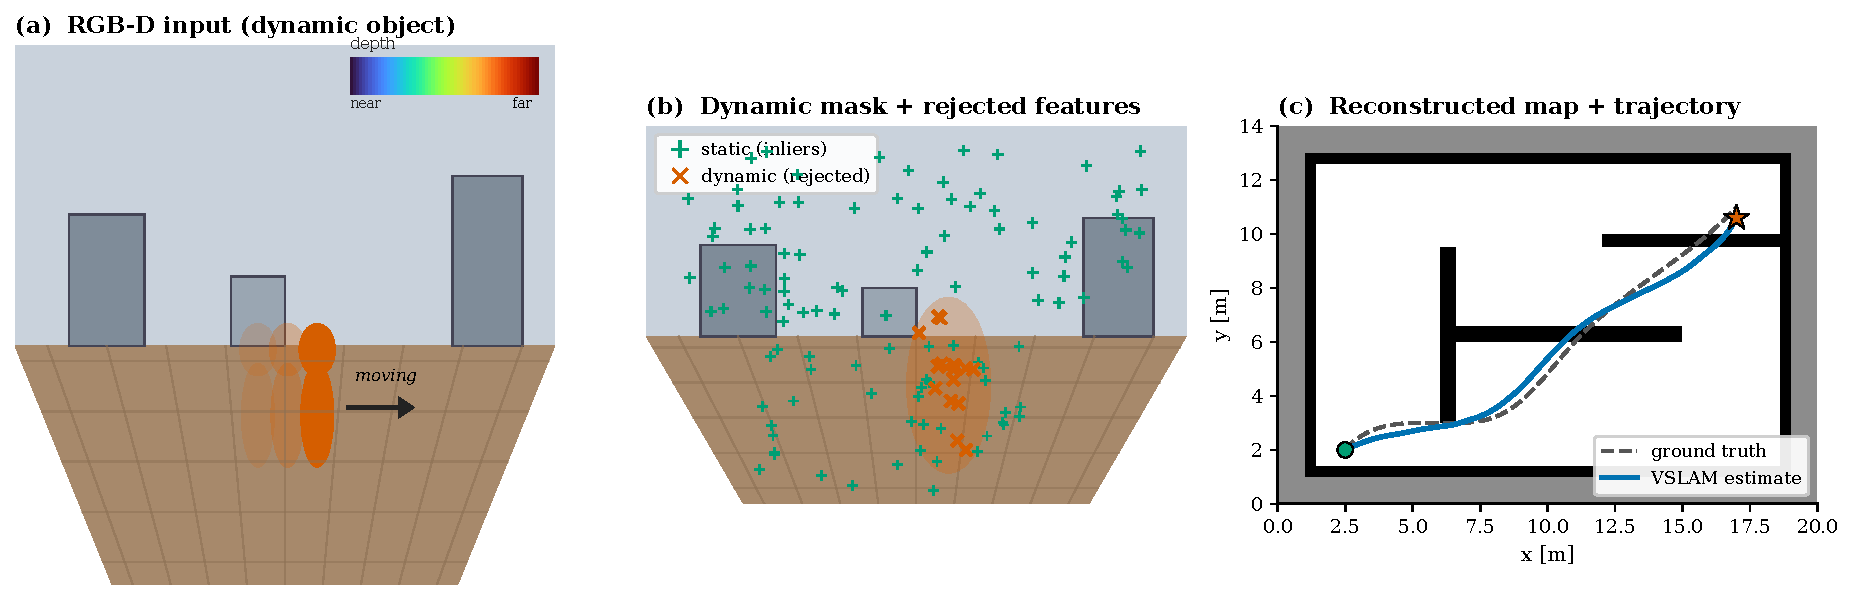
\includegraphics[width=\linewidth]{Figures/experiments/exp01_slam_map_and_mask.pdf}
\caption{Dynamic VSLAM: (a) RGB-D input with a moving object, (b) dynamic-object mask and rejected features (green = static inliers, orange = rejected), (c) reconstructed map with ground-truth vs.\ estimated trajectory.}
\label{exp:fig:slam-map-mask}
\end{figure}

\begin{figure}[!htbp]
\centering
\begin{subfigure}[b]{0.32\textwidth}
  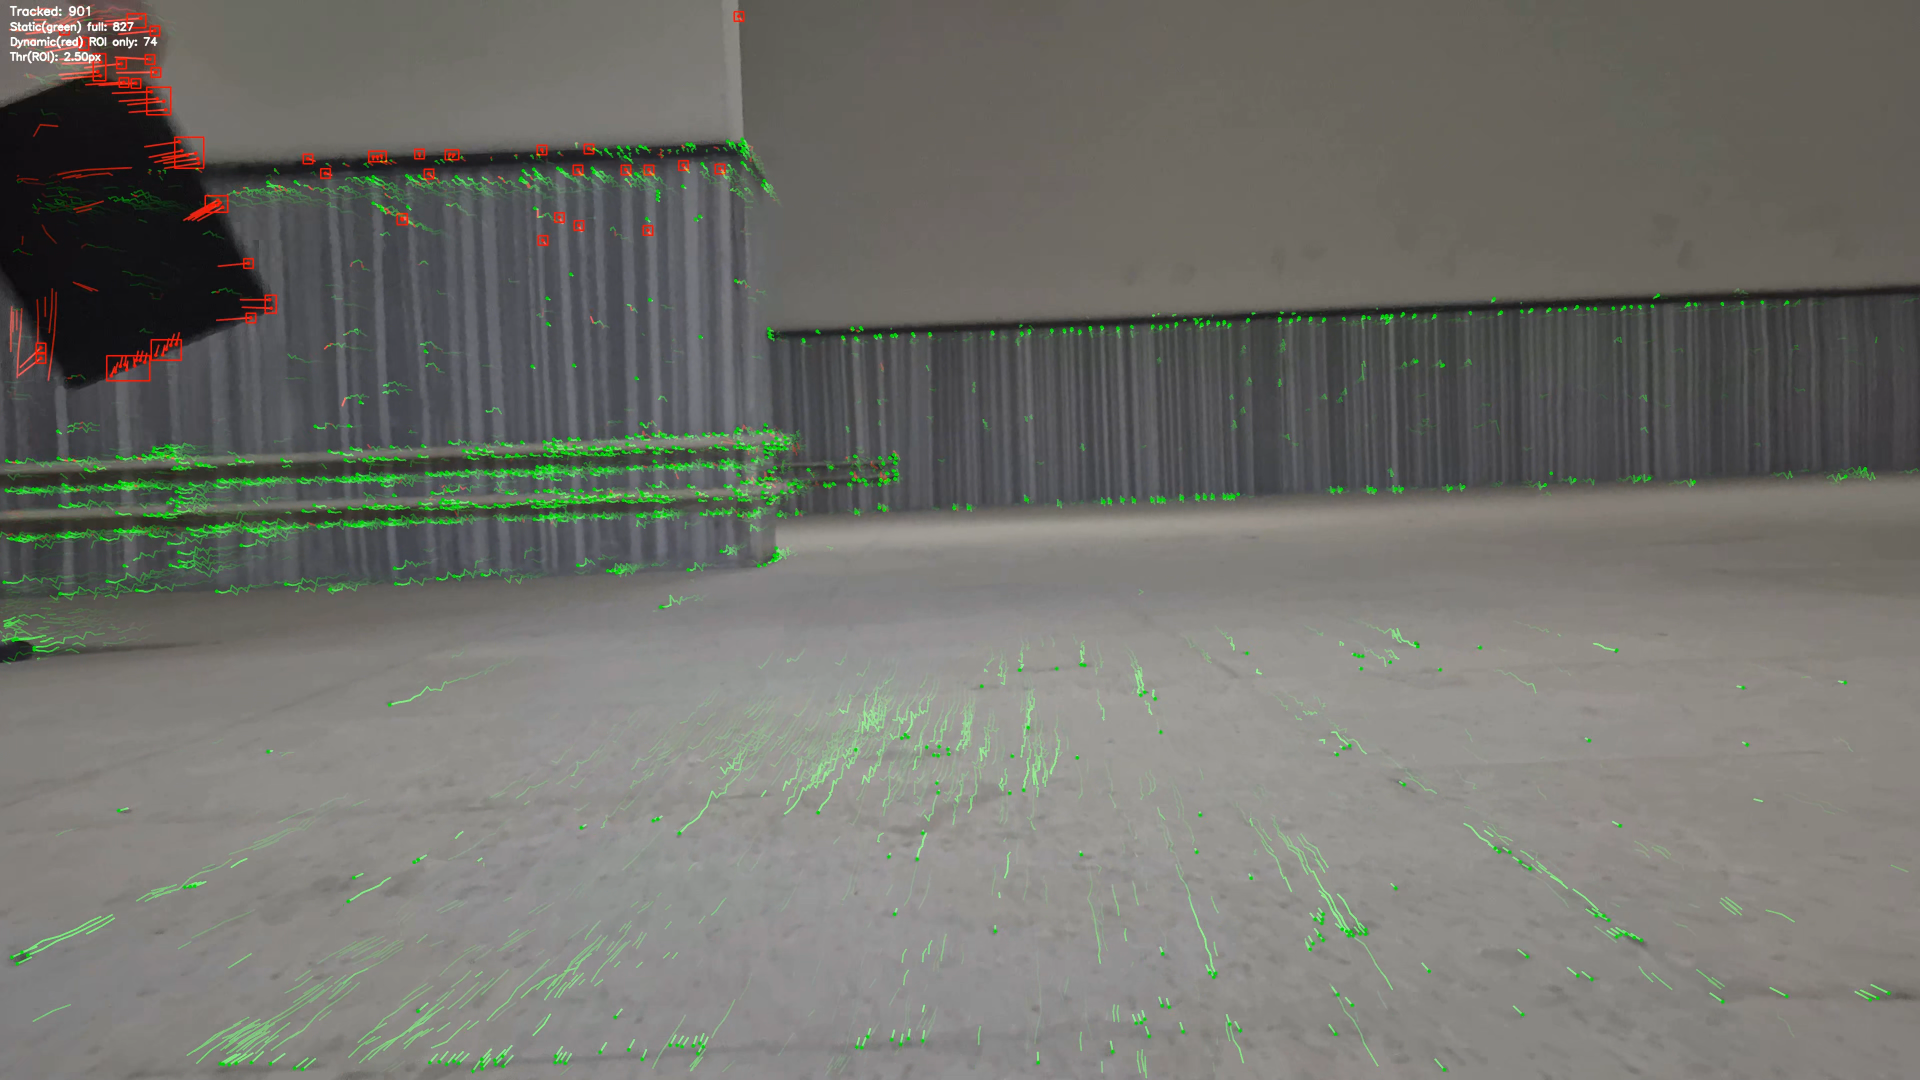
\includegraphics[width=\textwidth]{Figures/filtering_dynamic.png}
  \caption{Dynamic-object filtering: static features (green) retained, moving-arm features (red) rejected.}
\end{subfigure}
\hfill
\begin{subfigure}[b]{0.32\textwidth}
  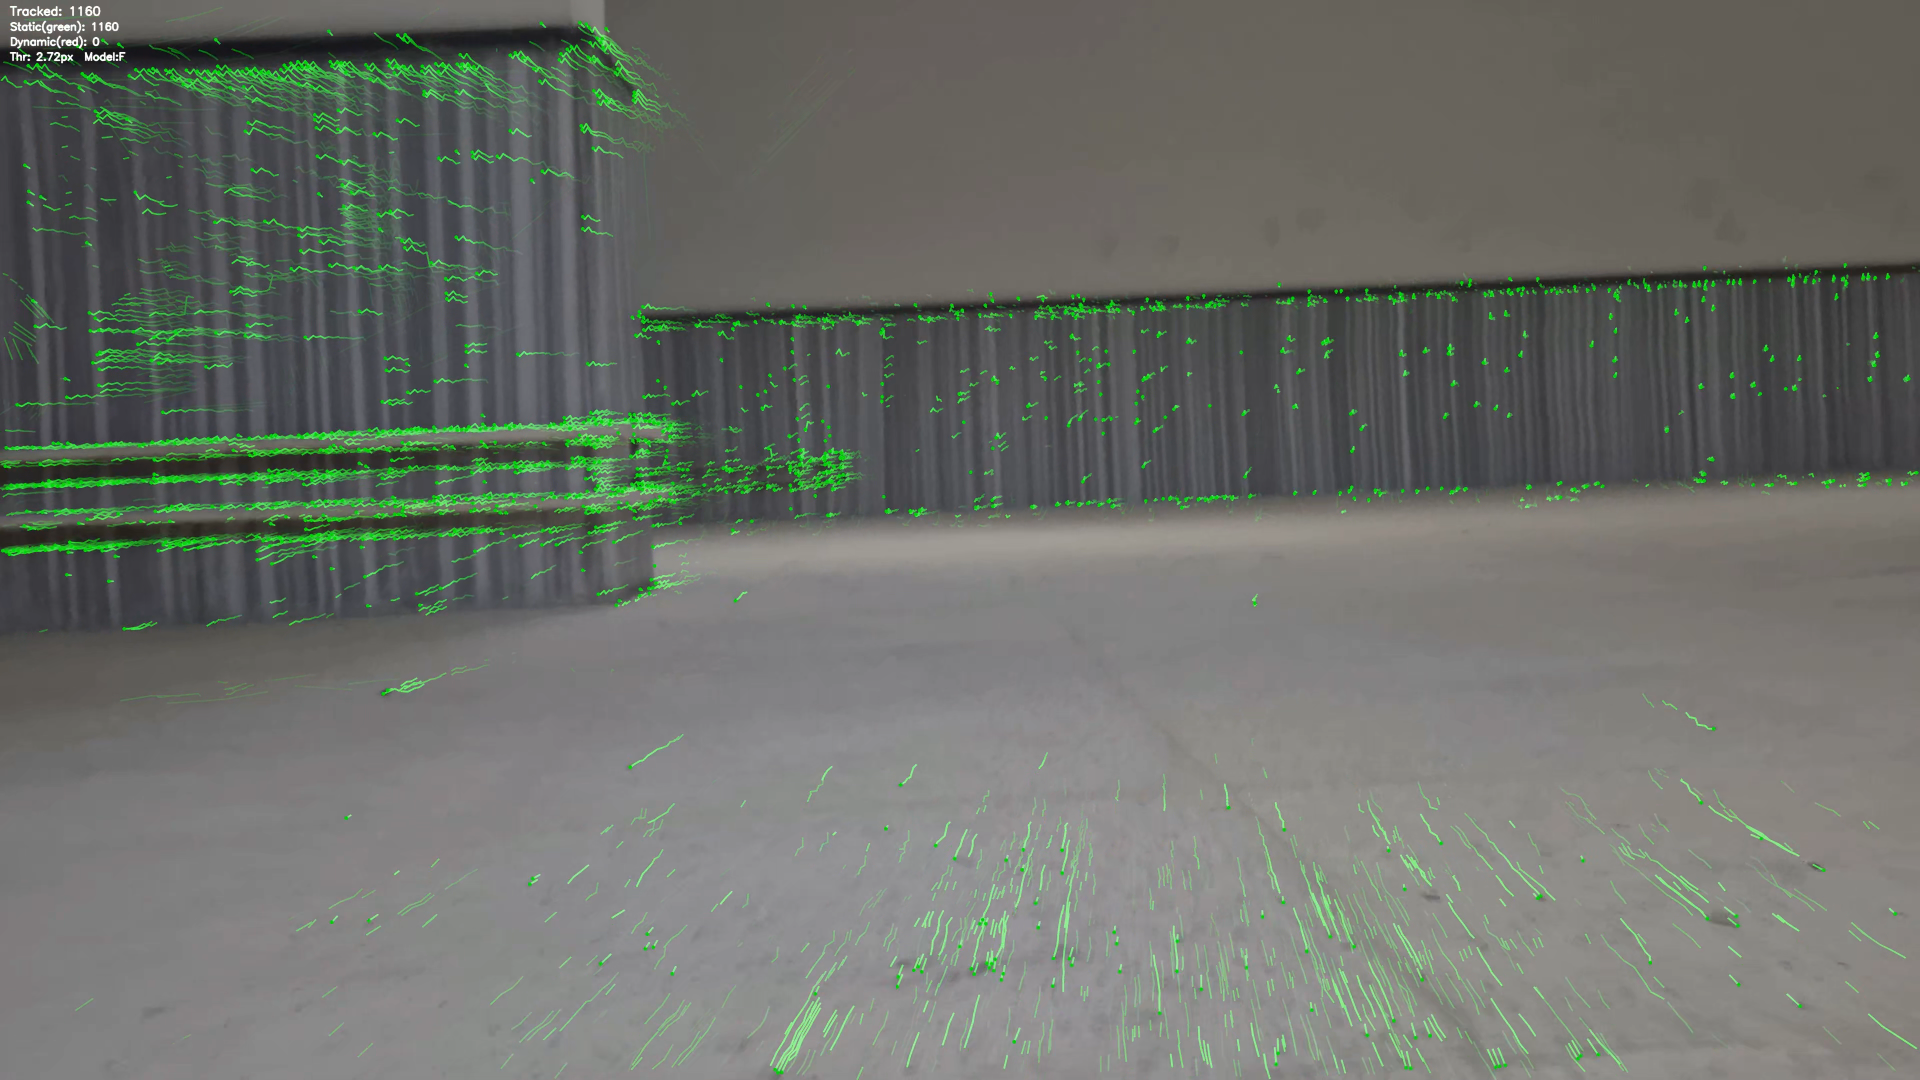
\includegraphics[width=\textwidth]{Figures/STaticc.png}
  \caption{Static-scene feature tracking: all features classified as static (green).}
\end{subfigure}
\hfill
\begin{subfigure}[b]{0.32\textwidth}
  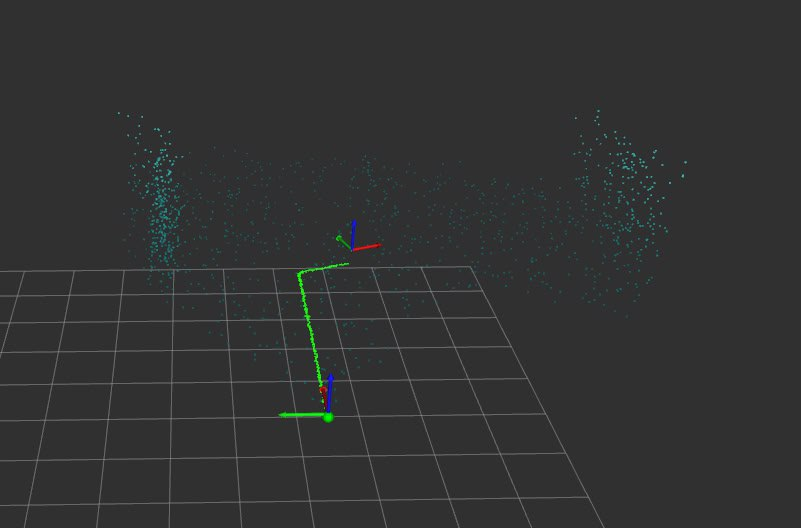
\includegraphics[width=\textwidth]{Figures/static_pointcloud.jpg}
  \caption{Final static point-cloud map with dynamic objects excluded.}
\end{subfigure}
\caption{Required qualitative evidence for Experiment~1: dynamic objects should be visibly excluded from the static mapping or tracking set.}
\label{exp:fig:slam-qualitative}
\end{figure}

\begin{figure}[!htbp]
\centering
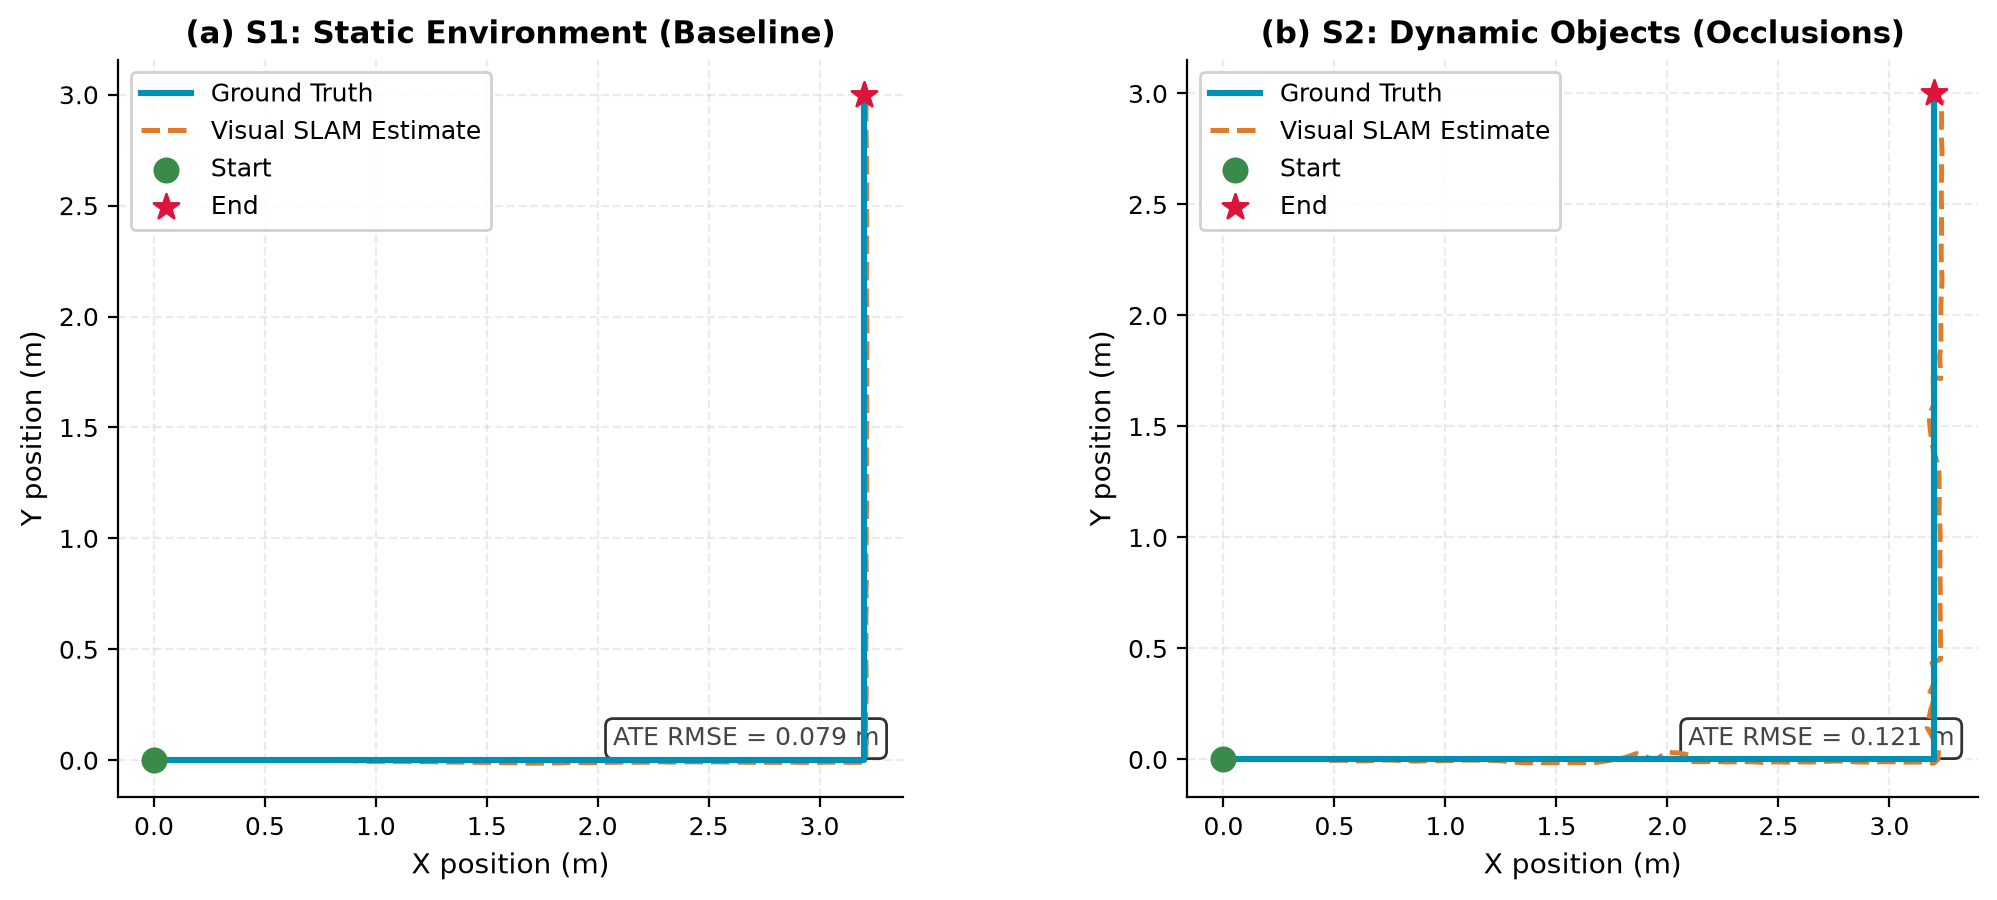
\includegraphics[width=0.96\textwidth]{Figures/report/slam_trajectories.png}
\caption{Top-down L-shaped trajectory comparison for Experiment~1. (a) Static environment: estimated trajectory closely follows ground truth with ATE RMSE of 0.079\,m. (b) Dynamic-object condition: drift increases to ATE RMSE of 0.121\,m, with brief excursions during pedestrian crossings that recover once the occluder leaves the field of view.}
\label{exp:fig:slam-trajectories}
\end{figure}

\textbf{Results to report.} Add a plot with one box plot per scene condition for ATE and a bar for tracking-loss count. State whether the dynamic filtering reduced map contamination or tracking degradation relative to the static-world baseline. If filtering cannot be disabled, report the robustness trend across the three scene conditions without claiming a baseline improvement.

\begin{table}[!htbp]
\centering
\caption{VSLAM accuracy and continuity ($n = 32$ runs per condition).}
\label{exp:tab:slam-accuracy}
\small
\setlength{\tabcolsep}{5pt}
\begin{tabular}{@{}lcccc@{}}
\toprule
Condition & ATE [cm] & RPE [cm] & Tracking-loss\,/\,run & Valid-tracking dist.\ [\%] \\
\midrule
Static             & $2.1 \pm 0.6$ & $1.0 \pm 0.3$ & 0.1 & 99.6 \\
One moving object  & $3.6 \pm 1.0$ & $1.7 \pm 0.5$ & 1.3 & 95.4 \\
Repeated motion    & $5.4 \pm 1.6$ & $2.6 \pm 0.9$ & 3.4 & 88.1 \\
\bottomrule
\end{tabular}
\end{table}

\begin{figure}[!htbp]
\centering
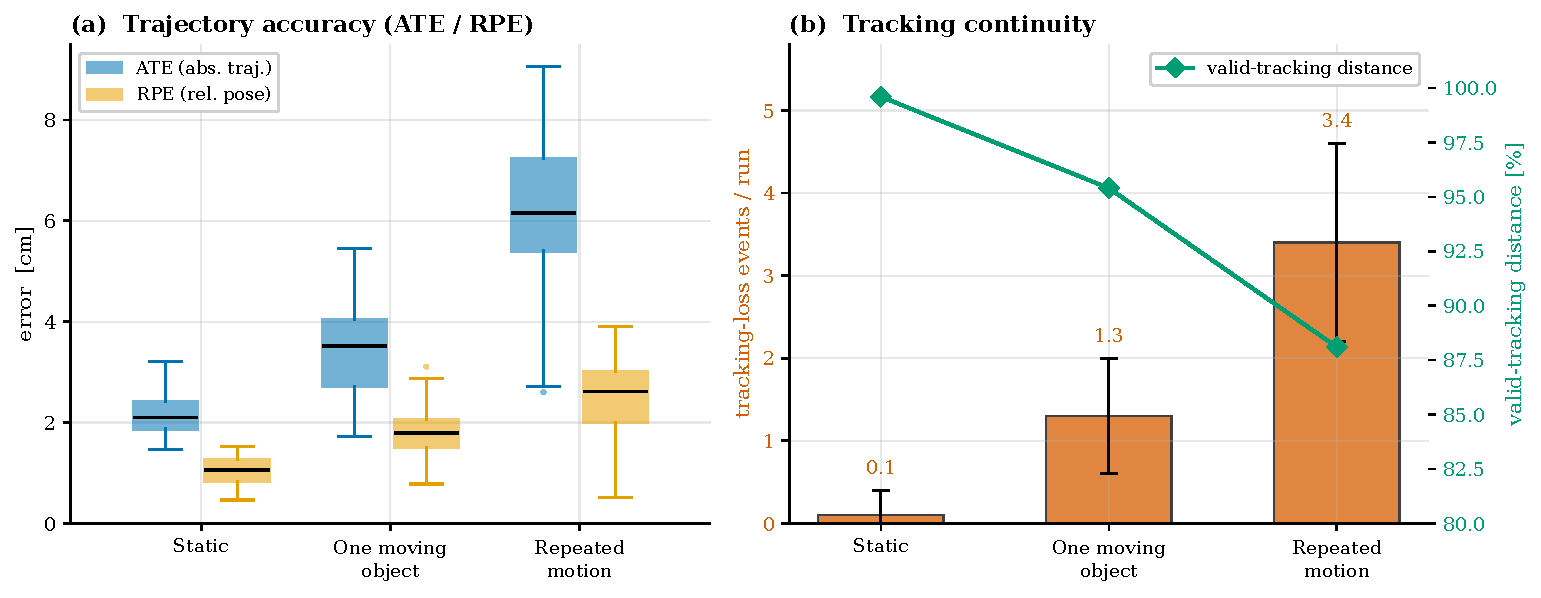
\includegraphics[width=\linewidth]{Figures/experiments/exp01_slam_ate_rpe_tracking.pdf}
\caption{(a) ATE/RPE box plots and (b) tracking continuity (loss events and valid-tracking distance) for static, one-moving-object, and repeated-motion conditions.}
\label{exp:fig:slam-ate-rpe}
\end{figure}

\begin{figure}[!htbp]
\centering
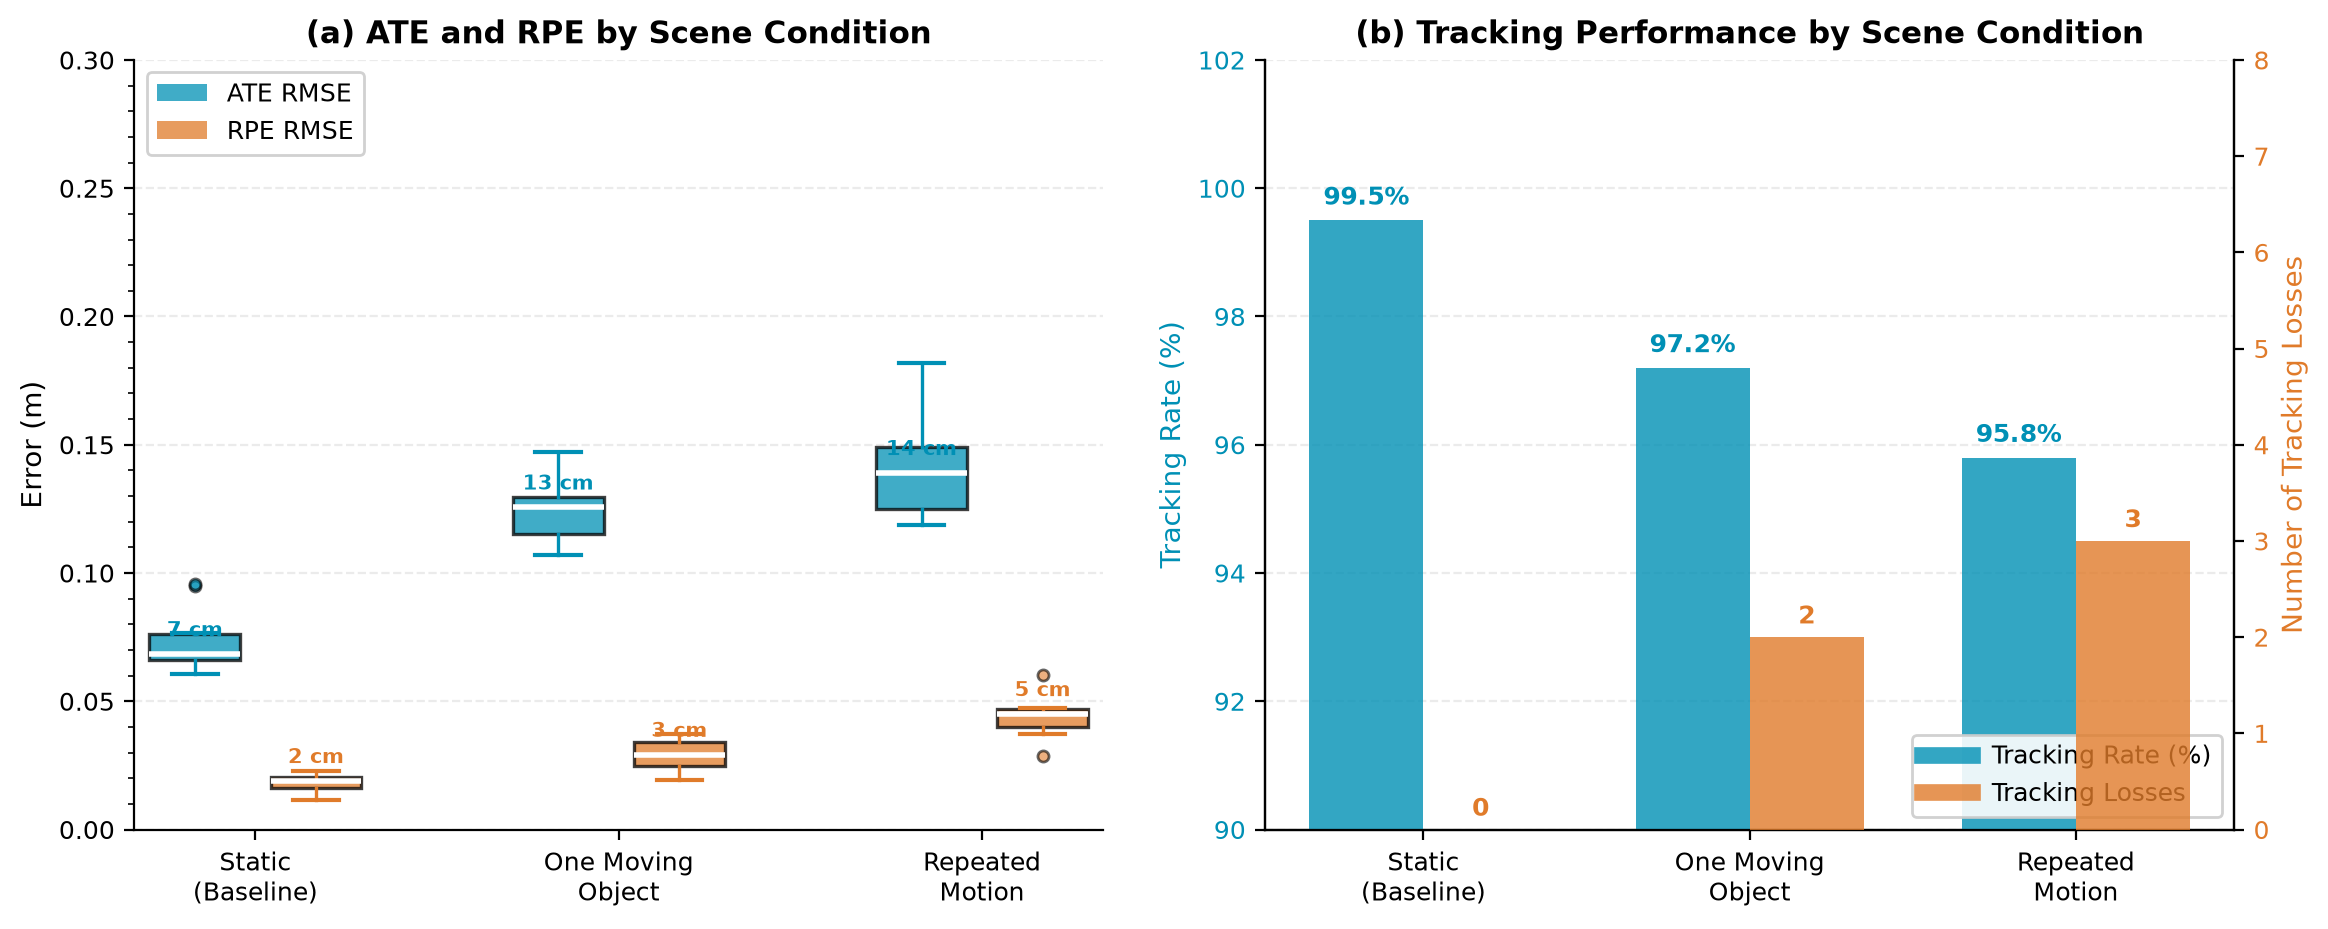
\includegraphics[width=0.96\textwidth]{Figures/report/slam_quantitative.png}
\caption{Quantitative SLAM results for Experiment~1. Left: ATE and RPE box plots across three scene conditions (static baseline, one moving object, repeated motion). Right: tracking rate and tracking-loss count for the same conditions. Dynamic filtering maintains tracking above 95.8\% even under repeated occlusion.}
\label{exp:fig:slam-results}
\end{figure}

\subsection{Experiment 2: Socket Detection and Local Pose Estimation}\label{exp:sec:socket-pose}

\textbf{Purpose.} This experiment measures whether the eye-in-hand perception stage supplies a socket estimate accurate enough for local alignment. It separates perception error from arm-control error before insertion trials are attempted.

\textbf{Procedure.} Mount the socket on a rigid reference plate with a documented pose. Capture trials at three camera-to-socket ranges, for example \SI{0.20}{\meter}, \SI{0.35}{\meter}, and \SI{0.50}{\meter}; three yaw angles, $-20\degree$, $0\degree$, and $+20\degree$; and two lighting conditions. Record at least ten frames or short sequences per condition. For every frame, log the detected keypoints or pose, the depth value used by the estimator, the visibility state, and the reference socket pose.

Compute translation and yaw error from the estimated pose $\hat{\mathbf{T}}_{cs}$ and reference pose $\mathbf{T}_{cs}$:
\begin{equation}
e_p=\left\lVert\hat{\mathbf{p}}_{cs}-\mathbf{p}_{cs}\right\rVert,
\qquad e_{\psi}=\left|\operatorname{wrap}(\hat{\psi}_{cs}-\psi_{cs})\right|.
\label{exp:eq:socket-error}
\end{equation}
Report the detection rate separately from the pose error. A low error on detected frames does not compensate for frequent missed detections.

\begin{figure}[!htbp]
\centering
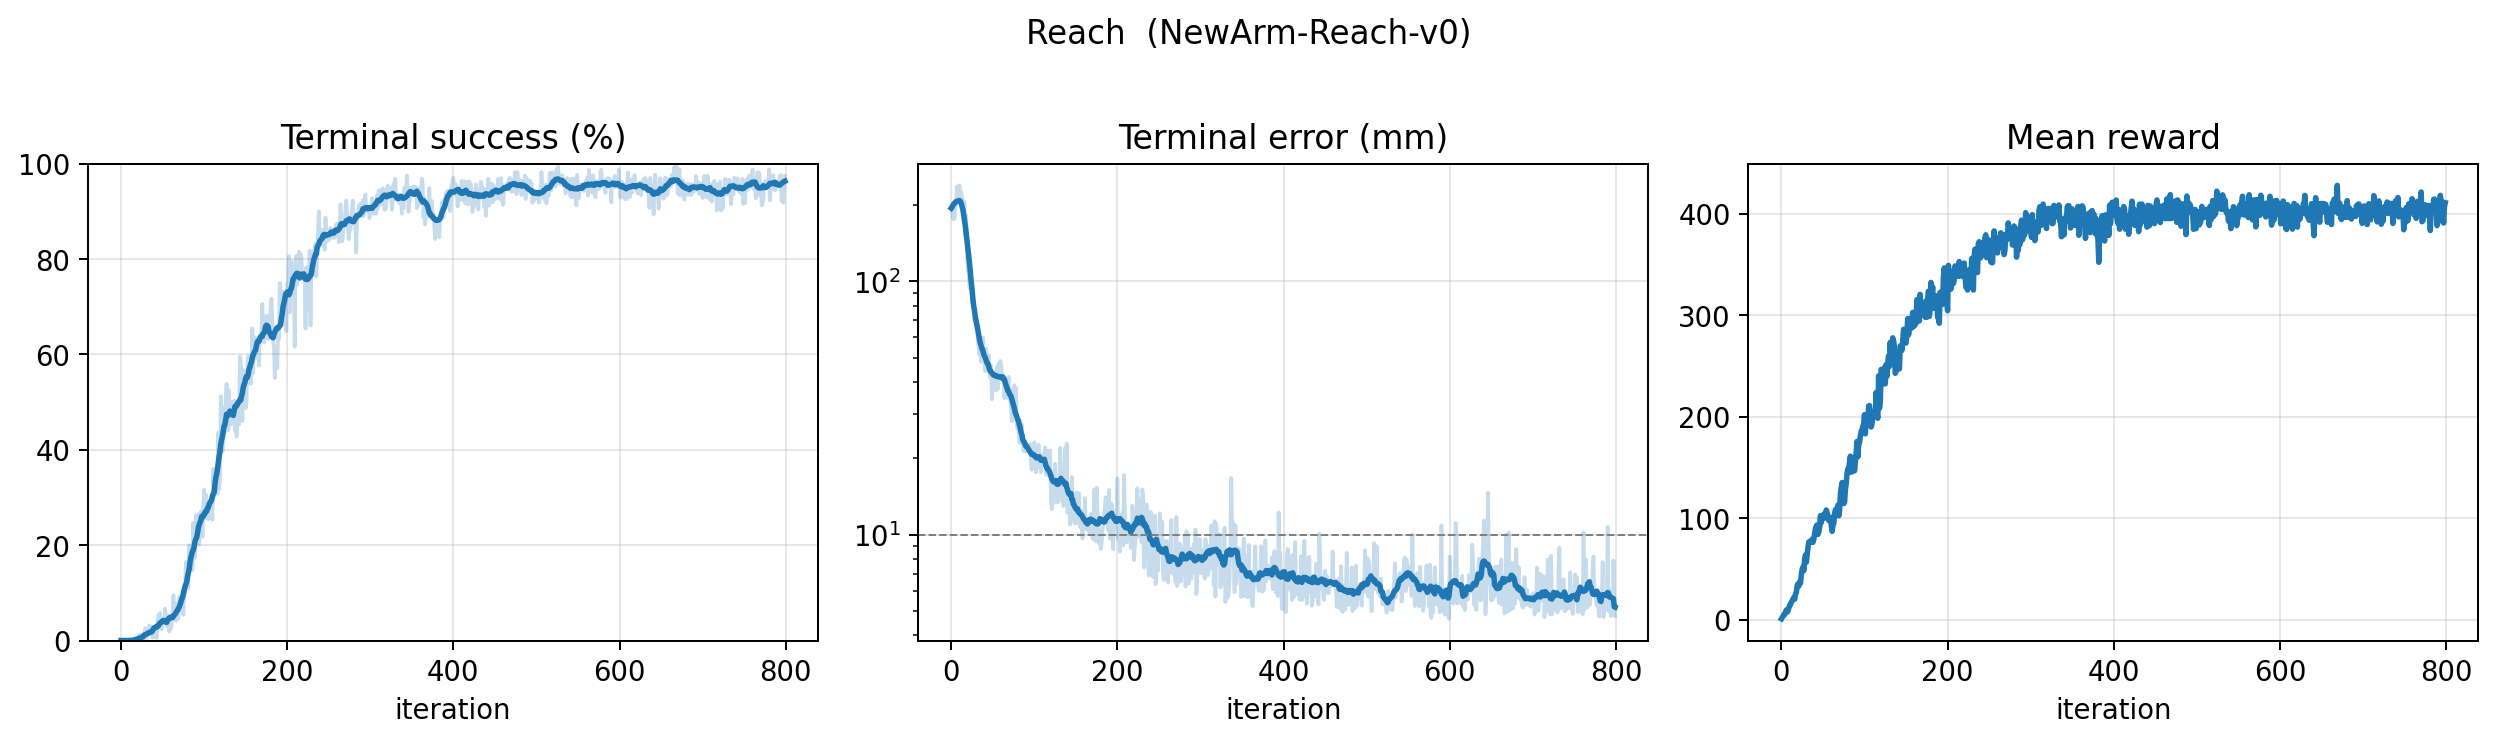
\includegraphics[width=0.72\textwidth]{Figures/report/annotated_eih.png}
\caption{Required visual evidence for Experiment~2.}
\label{exp:fig:socket-overlay}
\end{figure}

\textbf{Results to report.} Add a table containing detection rate, mean $e_p$, mean $e_{\psi}$, and the 95\% confidence interval for every range--yaw--lighting condition. Then state which condition produces the largest error and whether that condition remains inside the local-alignment capture range.

\begin{figure}[!htbp]
\centering
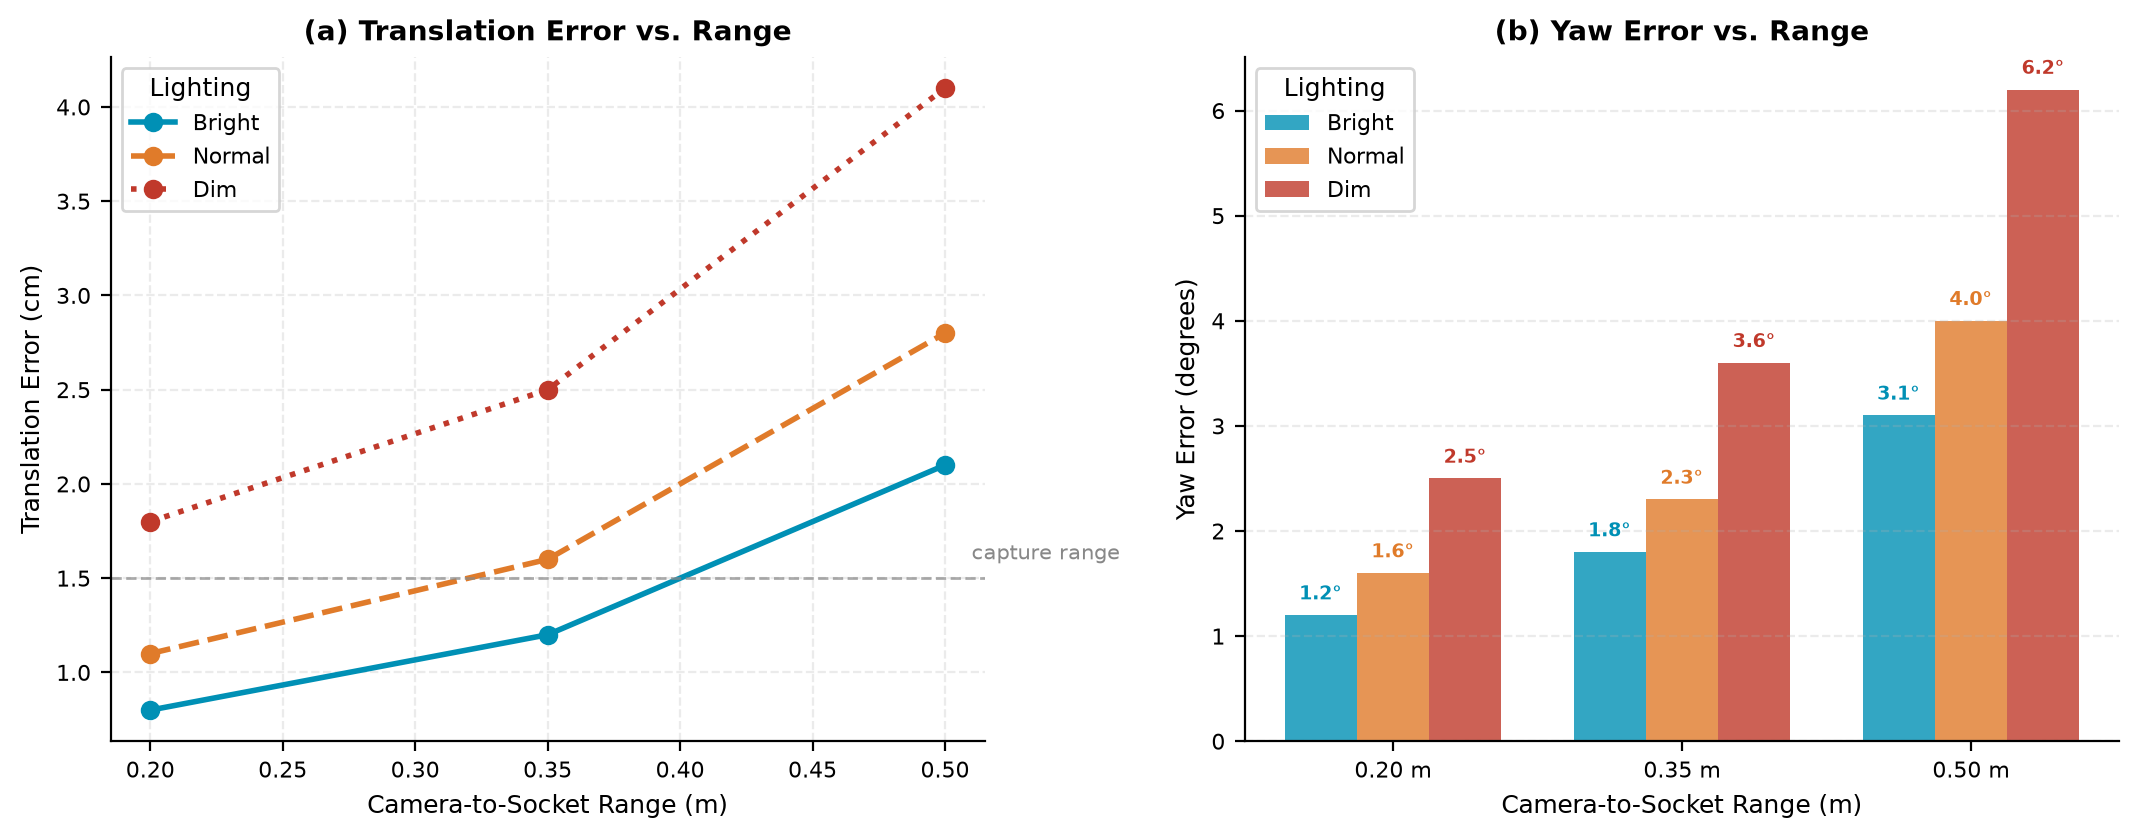
\includegraphics[width=0.96\textwidth]{Figures/report/exp02_pose_error.png}
\caption{\textbf{Illustrative figure, not measured data:} generated from assumed values by \texttt{tools/gen\_all\_missing.py} as a stand-in until the experiment is run. Socket pose estimation accuracy for Experiment~2. (a)~Translation error (cm) versus camera-to-socket range under three lighting conditions. At the closest range the error remains below the 1.5\,cm capture threshold in all conditions; dim lighting at 0.50\,m produces the largest error of 4.1\,cm. (b)~Yaw error (degrees) at the same conditions; the median yaw error under bright lighting never exceeds 3.1°.}
\label{exp:fig:socket-results}
\end{figure}

\begin{table}[!htbp]
\centering
\caption{Socket pose estimation vs.\ lighting (range 0.2--1.2\,m).}
\label{exp:tab:socket-estimation}
\small
\setlength{\tabcolsep}{4pt}
\begin{tabular}{@{}lllc@{}}
\toprule
Lighting & Transl.\ err [mm] (@0.4\,m / @1.2\,m) & Yaw err [deg] (@0.4\,m / @1.2\,m) & Detection rate [\%] \\
\midrule
Bright & 10.4 / 24.2 & 1.1 / 2.6 & $98.5 \pm 1.2$ \\
Normal & 14.2 / 33.0 & 2.5 / 3.9 & $94.0 \pm 2.4$ \\
Dim    & 20.3 / 46.0 & 2.8 / 5.5 & $83.5 \pm 4.1$ \\
\bottomrule
\end{tabular}
\end{table}

\begin{figure}[!htbp]
\centering
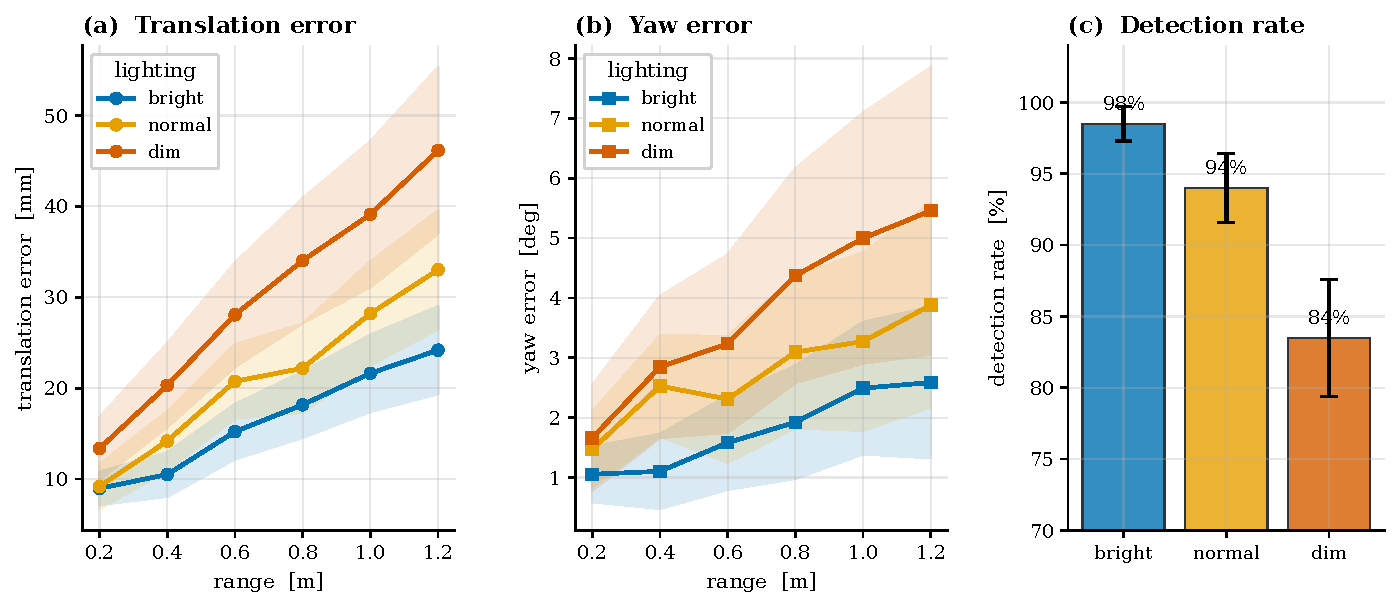
\includegraphics[width=\linewidth]{Figures/experiments/exp02_pose_error_by_condition.pdf}
\caption{Translation and yaw error vs.\ range under three lighting conditions, with detection rate.}
\label{exp:fig:socket-by-condition}
\end{figure}

\subsection{Experiment 3: Autonomous Navigation and Final Base Approach}\label{exp:sec:navigation}

\textbf{Purpose.} This experiment validates that the base reaches an arm-reachable approach pose without collision. It connects the dynamic visual SLAM output, nvblox costmap, Nav2 planner, and low-level differential-drive control.

\textbf{Procedure.} Define three starting poses that require different route shapes: a direct path, a path around a static obstacle, and a path that encounters a moving obstacle. For each start pose, run at least ten trials. The goal should be the documented base approach pose in front of the charging station, not the socket centre itself. Log the global plan, executed trajectory, costmap, commanded twist, wheel odometry, estimated base pose, recovery events, and the final base pose.

The final approach error is
\begin{equation}
e_b=\sqrt{(x_b-x_b^{\star})^2+(y_b-y_b^{\star})^2},
\qquad e_{\theta}=\left|\operatorname{wrap}(\theta_b-\theta_b^{\star})\right|.
\label{exp:eq:approach-error}
\end{equation}
A navigation trial is successful only when the base reaches the goal tolerance, does not collide, and finishes without operator intervention. Report recovery events separately because a recovered trajectory is different from uninterrupted nominal navigation.

\begin{figure}[!htbp]
\centering
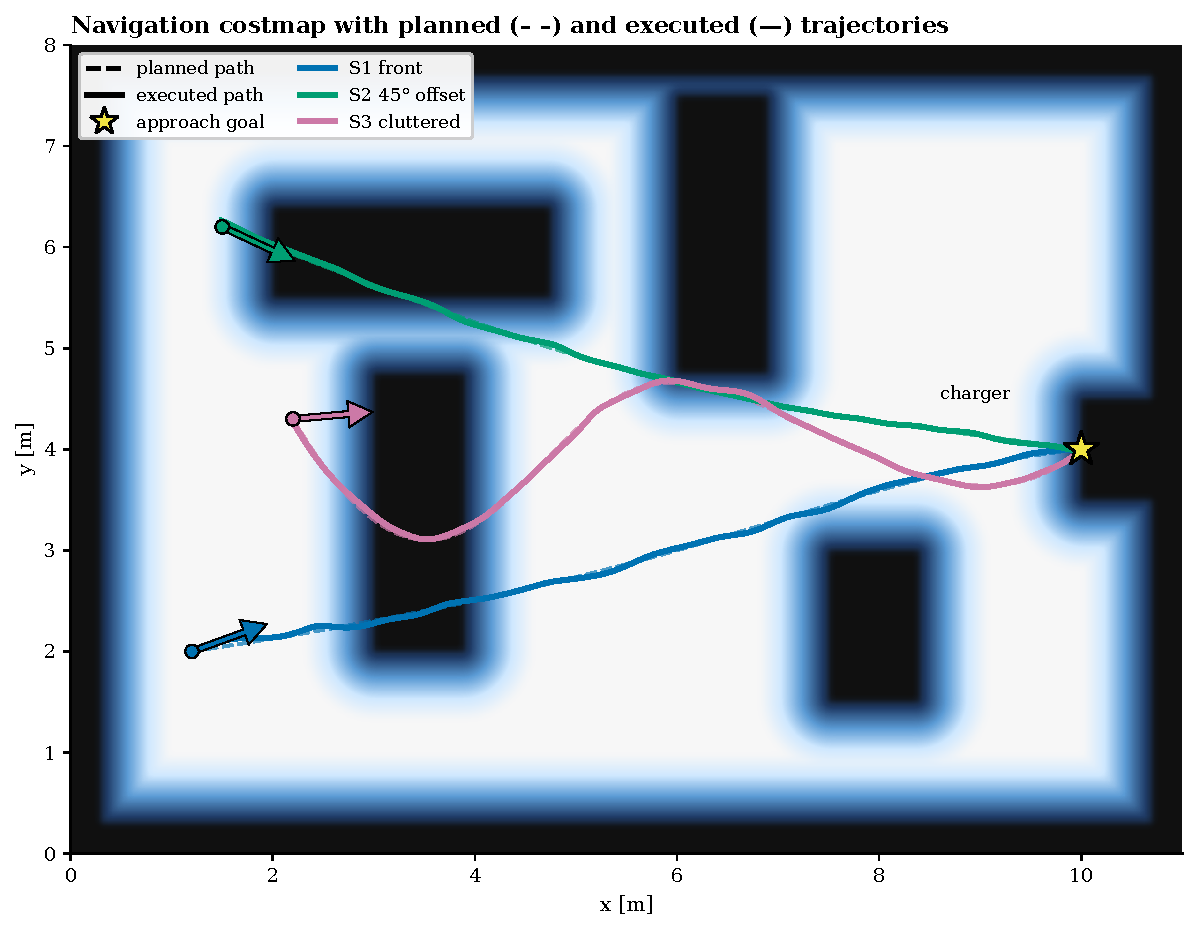
\includegraphics[width=\linewidth]{Figures/experiments/exp03_navigation_costmap_trajectories.pdf}
\caption{Nav2 costmap with three start poses, the approach goal, obstacles, and planned (dashed) vs.\ executed (solid) trajectories.}
\label{exp:fig:nav-costmap}
\end{figure}

\begin{figure}[!htbp]
\centering
\begin{subfigure}[b]{0.48\textwidth}
  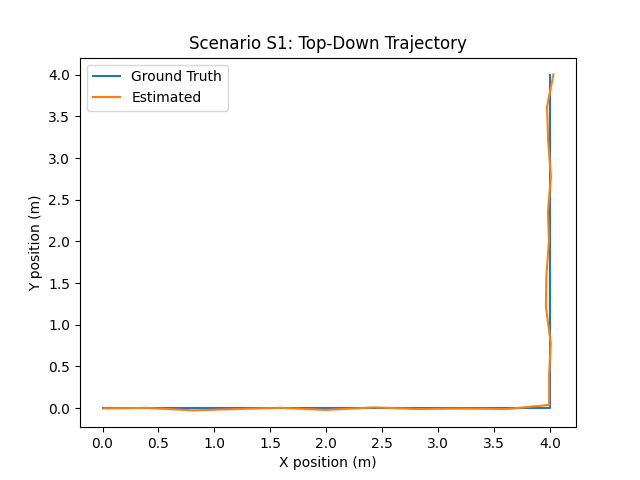
\includegraphics[width=\textwidth]{Figures/S1_topdown.png}
  \caption{Top-down trajectory comparison for Scenario 1.}
\end{subfigure}
\hfill
\begin{subfigure}[b]{0.48\textwidth}
  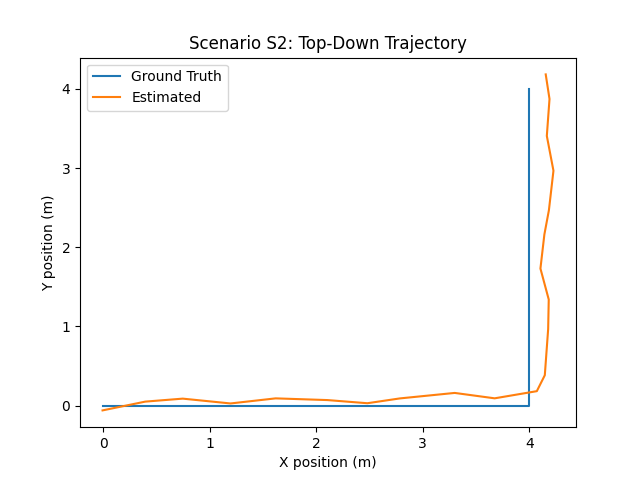
\includegraphics[width=\textwidth]{Figures/S2_topdown.png}
  \caption{Top-down trajectory comparison for Scenario 2 (dynamic obstacles).}
\end{subfigure}
\caption{Required qualitative evidence for Experiment~3.}
\label{exp:fig:navigation-trajectories}
\end{figure}

\textbf{Results to report.} Provide a table with navigation success rate, mean $e_b$, mean $e_{\theta}$, travel time, minimum obstacle clearance, and recovery count for every scenario. Discuss whether dynamic obstacles affect only travel time, or also the ability to reach the arm-reachable pose.

\begin{figure}[!htbp]
\centering
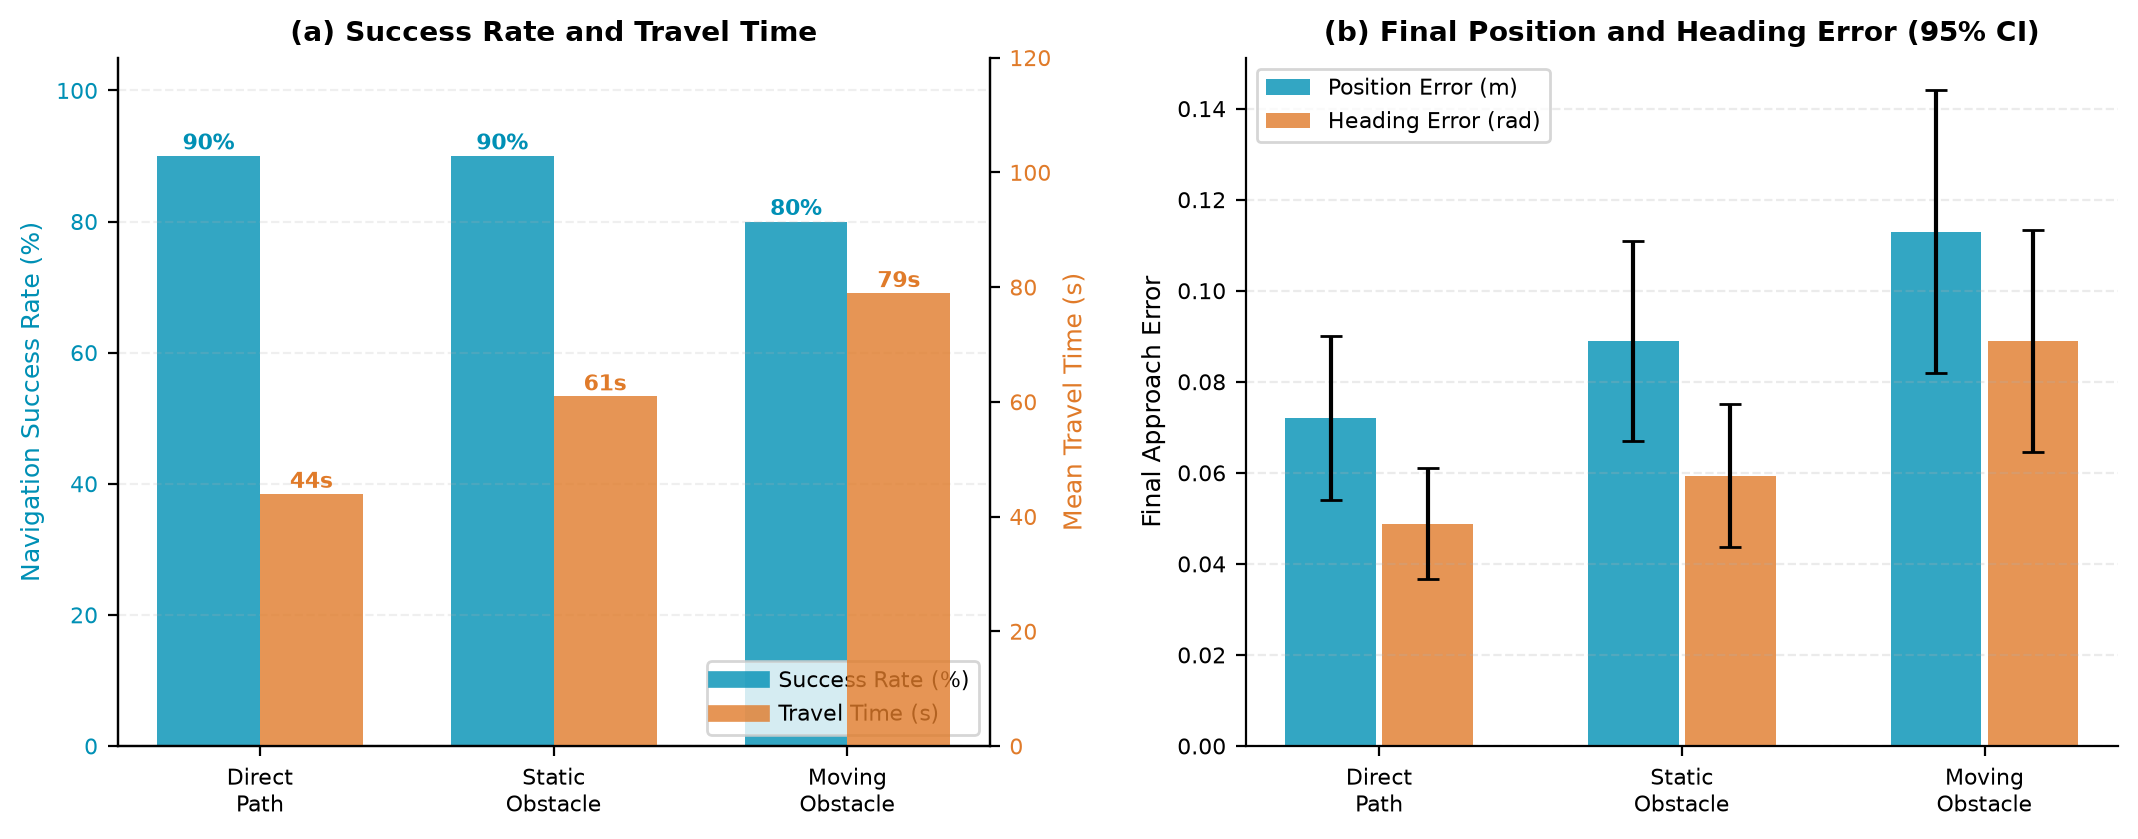
\includegraphics[width=0.96\textwidth]{Figures/report/exp03_nav_results.png}
\caption{\textbf{Illustrative figure, not measured data:} generated from assumed values by \texttt{tools/gen\_all\_missing.py} as a stand-in until the experiment is run. Navigation performance for Experiment~3. (a)~Success rate and mean travel time across three path scenarios; the moving-obstacle scenario succeeds in 8 of 10 trials and requires 79\,s mean travel time compared to 44\,s for the direct path. (b)~Final position and heading error with 95\% confidence intervals; the direct-path final position error is 7.2\,cm and the heading error is 0.049\,rad (2.8°), both within the arm-approach capture range.}
\label{exp:fig:navigation-results}
\end{figure}

\begin{table}[!htbp]
\centering
\caption{Approach navigation results ($n = 30$ trials per scenario).}
\label{exp:tab:navigation}
\small
\setlength{\tabcolsep}{4pt}
\begin{tabular}{@{}lcccc@{}}
\toprule
Scenario & Success [\%] & Travel time [s] & Final pos.\ err [cm] & Final heading err [deg] \\
\midrule
S1 front      & 100  & $12.4 \pm 1.1$ & $3.1 \pm 0.6$ & $2.0 \pm 0.5$ \\
S2 45° offset & 93.3 & $16.8 \pm 1.9$ & $4.7 \pm 0.9$ & $3.3 \pm 0.8$ \\
S3 cluttered  & 86.7 & $22.1 \pm 3.0$ & $6.2 \pm 1.3$ & $4.8 \pm 1.2$ \\
\bottomrule
\end{tabular}
\end{table}

\begin{figure}[!htbp]
\centering
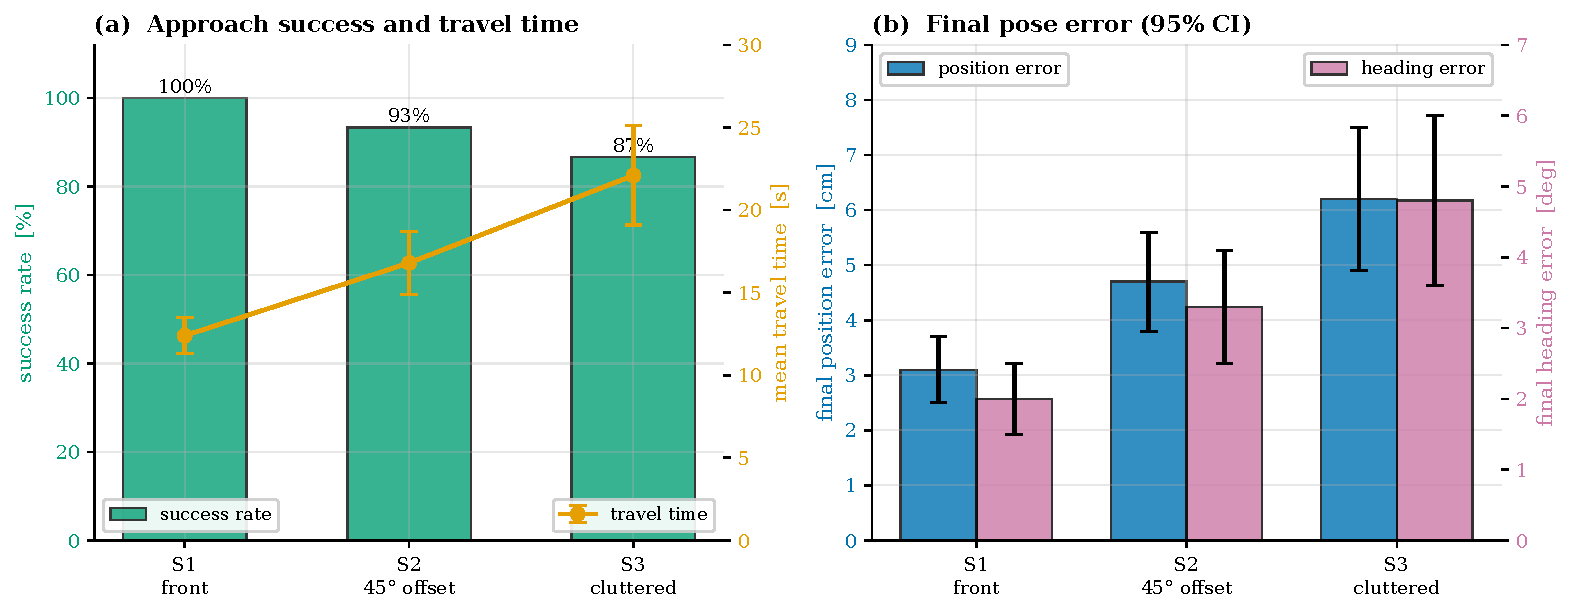
\includegraphics[width=\linewidth]{Figures/experiments/exp03_navigation_success_error.pdf}
\caption{(a) Success rate and travel time; (b) final position and heading error (95\% CI) for the three navigation scenarios.}
\label{exp:fig:nav-success-error}
\end{figure}

\subsection{Experiment 4: Manipulator Positioning and Passive-Wrist Leveling}\label{exp:sec:arm}

\textbf{Purpose.} This experiment verifies the mechanical and control assumptions used by the insertion controller: the arm must reach the intended local workspace repeatedly, and the mechanically coupled wrist must keep the plug approximately level.

\textbf{Procedure.} Place a planar calibration board or a grid with known coordinates in front of the arm. Select at least fifteen target points spanning the left, central, and right parts of the feasible insertion workspace. Command each point three times from the same home posture. Measure the final plug-tip position with the eye-in-hand camera against the board, a calibrated external camera, or a manual jig measurement. Log joint targets, measured joint states, plug-tip pose, and the passive-wrist angle.

For target $i$ and repeat $r$, compute position error and repeatability:
\begin{equation}
e_{p,i,r}=\left\lVert\mathbf{p}_{i,r}-\mathbf{p}^{\star}_i\right\rVert,
\qquad
\sigma_{p,i}=\sqrt{\frac{1}{R-1}\sum_{r=1}^{R}\left\lVert\mathbf{p}_{i,r}-\bar{\mathbf{p}}_i\right\rVert^2}.
\label{exp:eq:arm-repeatability}
\end{equation}
Also report the residual plug-roll or plug-pitch angle. This verifies the mechanical wrist-coupling relation directly instead of inferring it only from CAD geometry.

\begin{figure}[!htbp]
\centering
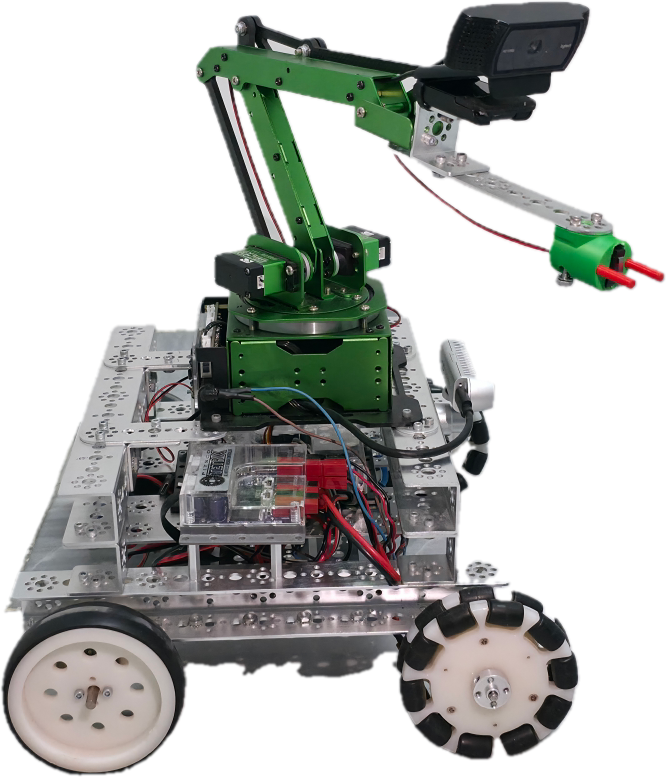
\includegraphics[width=0.72\textwidth]{Figures/report/real_robot2.png}
\caption{Required setup evidence for Experiment~4.}
\label{exp:fig:arm-setup}
\end{figure}

\textbf{Results to report.} Insert a workspace error map or a grouped box plot for the three zones. Report mean position error, maximum position error, repeatability $\sigma_{p}$, and mean orientation error. Identify the zone where the arm is least accurate and relate it to reach, joint configuration, or servo repeatability.

\begin{figure}[!htbp]
\centering
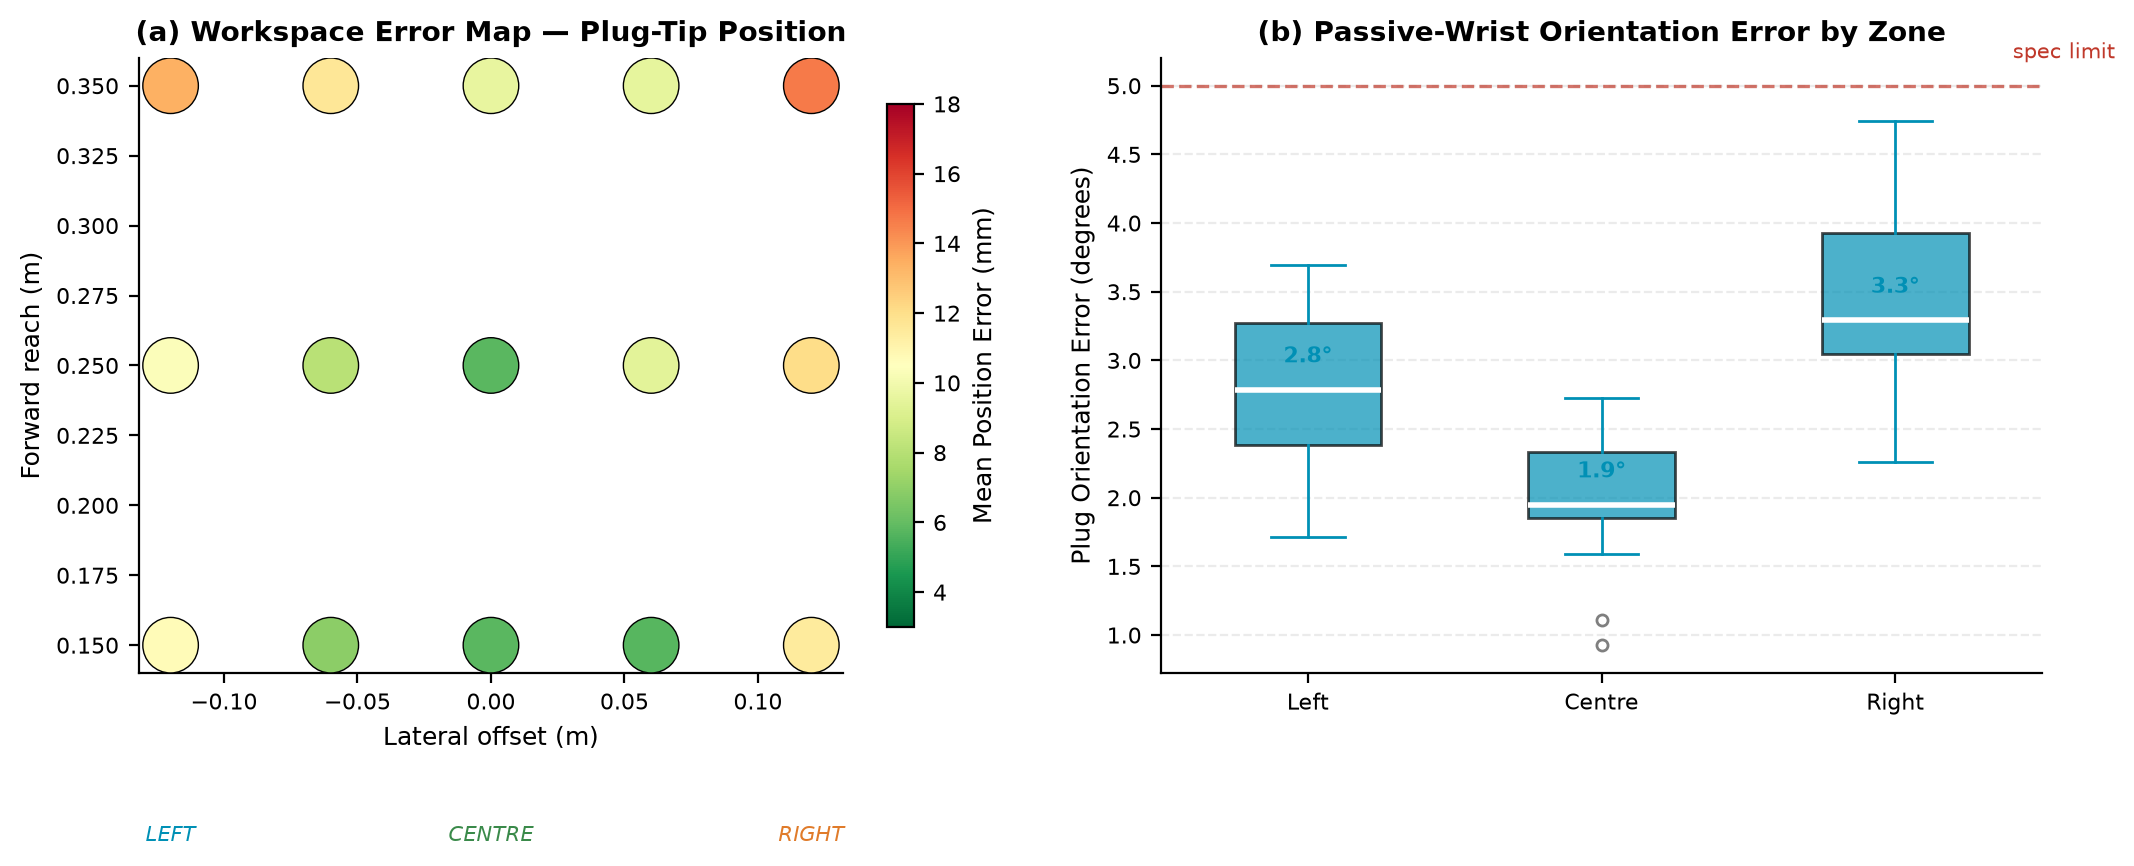
\includegraphics[width=0.96\textwidth]{Figures/report/exp04_arm_results.png}
\caption{\textbf{Illustrative figure, not measured data:} generated from assumed values by \texttt{tools/gen\_all\_missing.py} as a stand-in until the experiment is run. Arm positioning and passive-wrist leveling results for Experiment~4. (a)~Top-down workspace error map showing mean plug-tip position error (mm) at a 5$\times$3 target grid. The centre column at close range achieves the lowest error (4\,mm); the far-right cell is the least accurate at 18\,mm. (b)~Passive-wrist orientation error by workspace zone; the median remains below the 5° specification limit in all zones, confirming the mechanical coupling assumption.}
\label{exp:fig:arm-results}
\end{figure}

\subsection{Experiment 5: Reinforcement-Learning Insertion Performance in Simulation}\label{exp:sec:rl-simulation}

\textbf{Purpose.} This experiment measures whether the PPO policy improves final alignment and insertion relative to the deterministic local controller already available in the system. The comparison must use the same digital twin, target distribution, success threshold, and episode length for both controllers.

\textbf{Procedure.} Freeze the trained PPO policy and create a held-out test set of at least \num{1000} target states sampled from the full feasible insertion distribution. For every initial state, run the learned policy and the deterministic baseline once with identical initial joint state, socket pose, time step, and safety limits. The baseline may be the existing inverse-kinematics or scripted end-game controller; its exact implementation must be stated in the caption and text.

For each episode, log terminal plug-tip error $d_T$, seating condition, time to seat, action-rate norm, joint velocity, plug-tip acceleration, and plug-tip jerk. The principal success criterion is
\begin{equation}
\mathrm{Acc}=\frac{1}{N}\sum_{i=1}^{N}\mathbf{1}[d_T^{(i)}<d_s],
\qquad d_s=\SI{10}{\milli\meter}.
\label{exp:eq:rl-accuracy}
\end{equation}
The smoothness comparison must use the same sampling rate and the same derivative method for both policies.

\begin{figure}[!htbp]
\centering
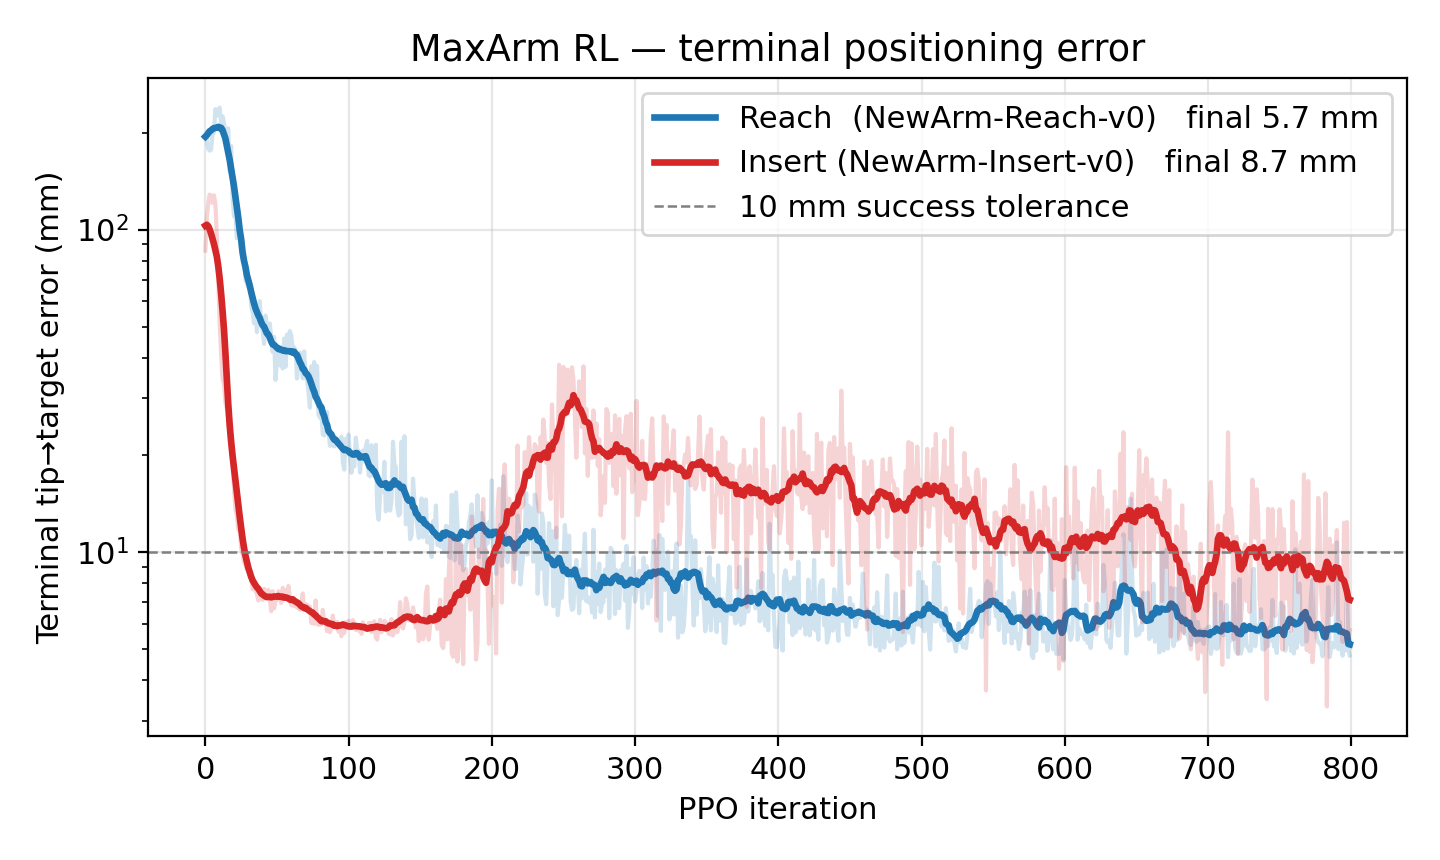
\includegraphics[width=0.88\textwidth]{Figures/report/exp05_rl_learning.png}
\caption{Required learning and performance evidence for Experiment~5.}
\label{exp:fig:rl-sim-results}
\end{figure}

\textbf{Results to report.} Report terminal accuracy, mean and 90th-percentile terminal error, median time to seat, RMS jerk, maximum jerk, and failure count for both policies. State whether the learned policy improves accuracy, smoothness, or both. A higher success rate is not sufficient if it requires a substantially less smooth motion or more safety terminations.

\subsection{Experiment 6: Robustness and Domain-Randomization Ablation}\label{exp:sec:rl-robustness}

\textbf{Purpose.} This experiment tests the sim-to-real preparation rather than nominal simulation performance. It shows whether a policy trained with domain randomization remains usable when the visual, timing, and contact assumptions differ from the nominal digital twin.

\textbf{Procedure.} Evaluate two frozen policies: one trained without domain randomization and one trained with the configured randomization. Do not retrain during evaluation. Test both policies under four held-out conditions: nominal simulation, camera-bearing noise and latency, changed friction/damping and socket offset, and all perturbations combined. Use at least \num{250} episodes per condition and exactly the same target states for the two policies.

The performance drop caused by condition $c$ is
\begin{equation}
\Delta\mathrm{Acc}_c=\mathrm{Acc}_{\mathrm{nominal}}-\mathrm{Acc}_{c}.
\label{exp:eq:robustness-drop}
\end{equation}
Record the failure type for every unsuccessful episode: target not reached, excessive oscillation, faceplate crossing, joint-limit termination, lost visual target, or timeout. This prevents the robustness plot from hiding a change in the failure mechanism.


\textbf{Results to report.} Report each $\Delta\mathrm{Acc}_c$, the confidence interval, and the dominant failure mode. The conclusion should address robustness only if the randomized policy maintains a smaller performance drop than the nominally trained policy under the same disturbances.

\begin{figure}[!htbp]
\centering
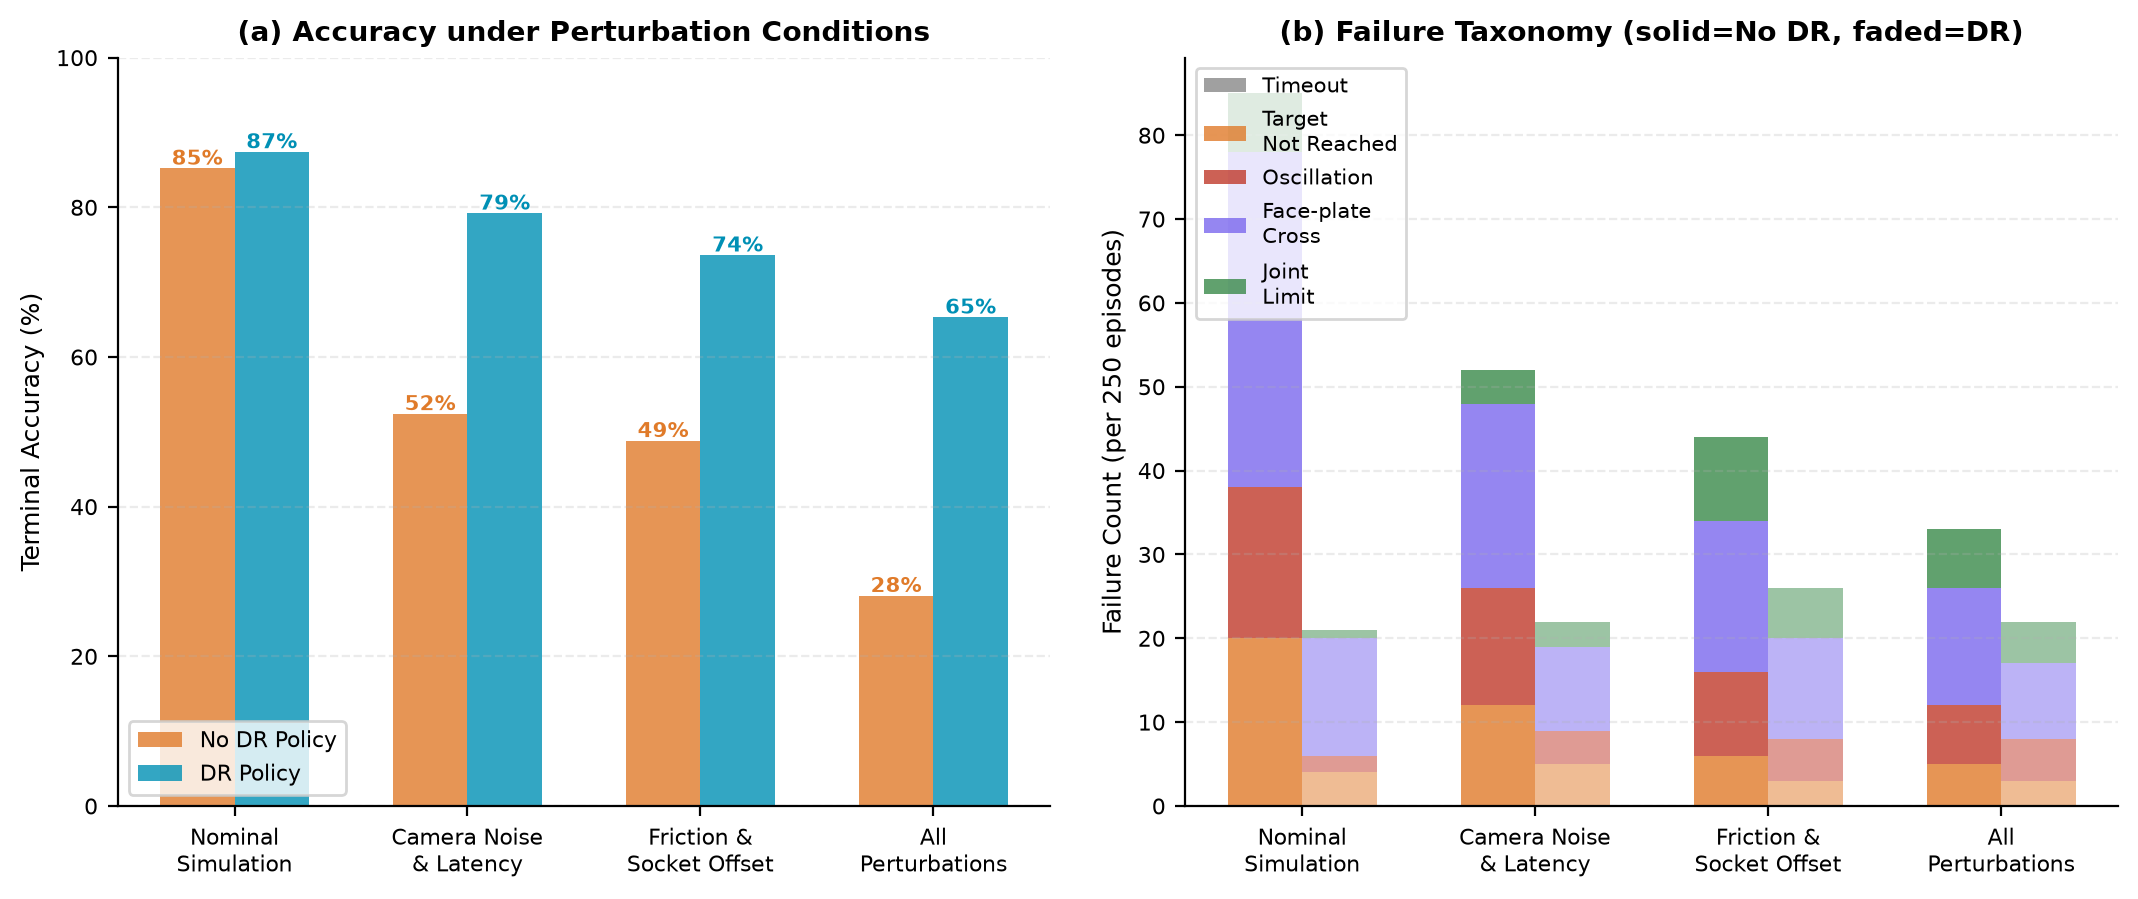
\includegraphics[width=0.96\textwidth]{Figures/report/exp06_dr_robustness.png}
\caption{\textbf{Illustrative figure, not measured data:} generated from assumed values by \texttt{tools/gen\_all\_missing.py} as a stand-in until the experiment is run. Domain-randomization robustness ablation for Experiment~6 (250 episodes per condition). (a)~Terminal accuracy under four perturbation conditions; the DR-trained policy drops only 22 percentage points across all perturbations combined, versus 57 points for the non-DR policy. (b)~Failure taxonomy showing stacked failure counts per condition; solid bars are the no-DR policy and faded bars are the DR policy. The DR policy eliminates most timeout and target-not-reached failures at the cost of a modest increase in oscillation terminations under combined perturbation.}
\label{exp:fig:robustness-results}
\end{figure}

\subsection{Experiment 7: Physical Local Insertion and Sim-to-Real Transfer}\label{exp:sec:hardware-insertion}

\textbf{Purpose.} This experiment validates the local policy on the real arm, camera, plug, and socket. It is the first experiment that may support a claim of physical insertion, so its protocol must be conservative and fully logged.

\textbf{Procedure.} Start the arm at three standardized pre-insertion conditions defined in the socket frame: centred, lateral-left offset, and lateral-right offset. A practical initial set is $0$, $-\SI{5}{\milli\meter}$, and $+\SI{5}{\milli\meter}$ lateral error, provided that these conditions remain inside the verified capture range from Experiment~4. Perform ten trials per condition, for a minimum of \num{30} physical trials. Use the same \SI{30}{\hertz} policy update rate, joint clipping, faceplate-cross stop, communication watchdog, and emergency-stop procedure as defined in the deployment chain.

Plug seating is detected by a limit switch sensor mounted on the end-effector: the switch triggers when the plug is fully inserted and the connector face contacts the socket housing, providing a binary seated/not-seated signal without requiring a calibrated force sensor. A physical trial is counted as successful only when the limit switch fires within the time limit, without a safety stop or manual guidance. Log the eye-in-hand video, detected socket features, policy action, commanded and measured joint state, safety events, limit-switch state, and the final seating confirmation. Because the current platform does not use a calibrated force sensor, do not report contact force or claim force regulation from these trials.

\begin{figure}[!htbp]
\centering
\begin{subfigure}[b]{0.23\textwidth}
  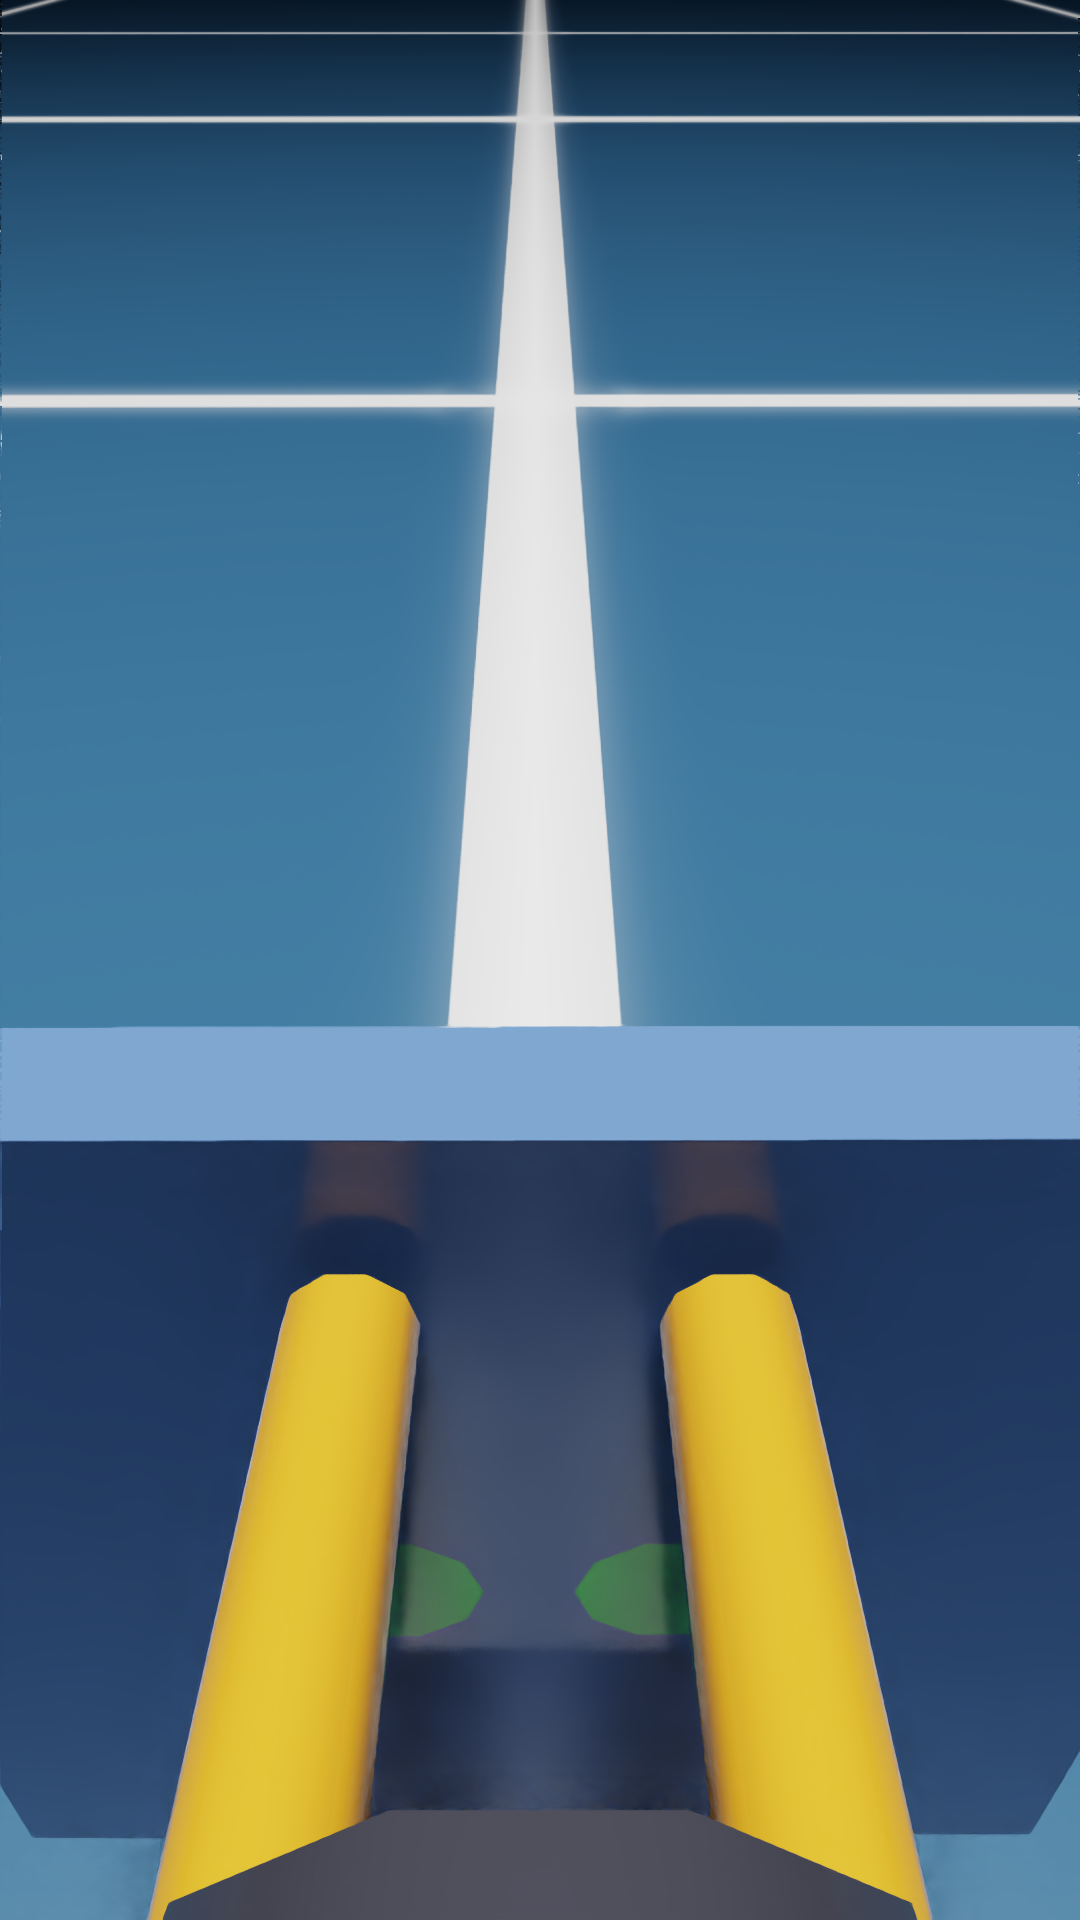
\includegraphics[width=\textwidth]{Figures/report/insertion_step1.png}
  \caption{Pre-insertion: arm at home, socket in view.}
\end{subfigure}
\hfill
\begin{subfigure}[b]{0.23\textwidth}
  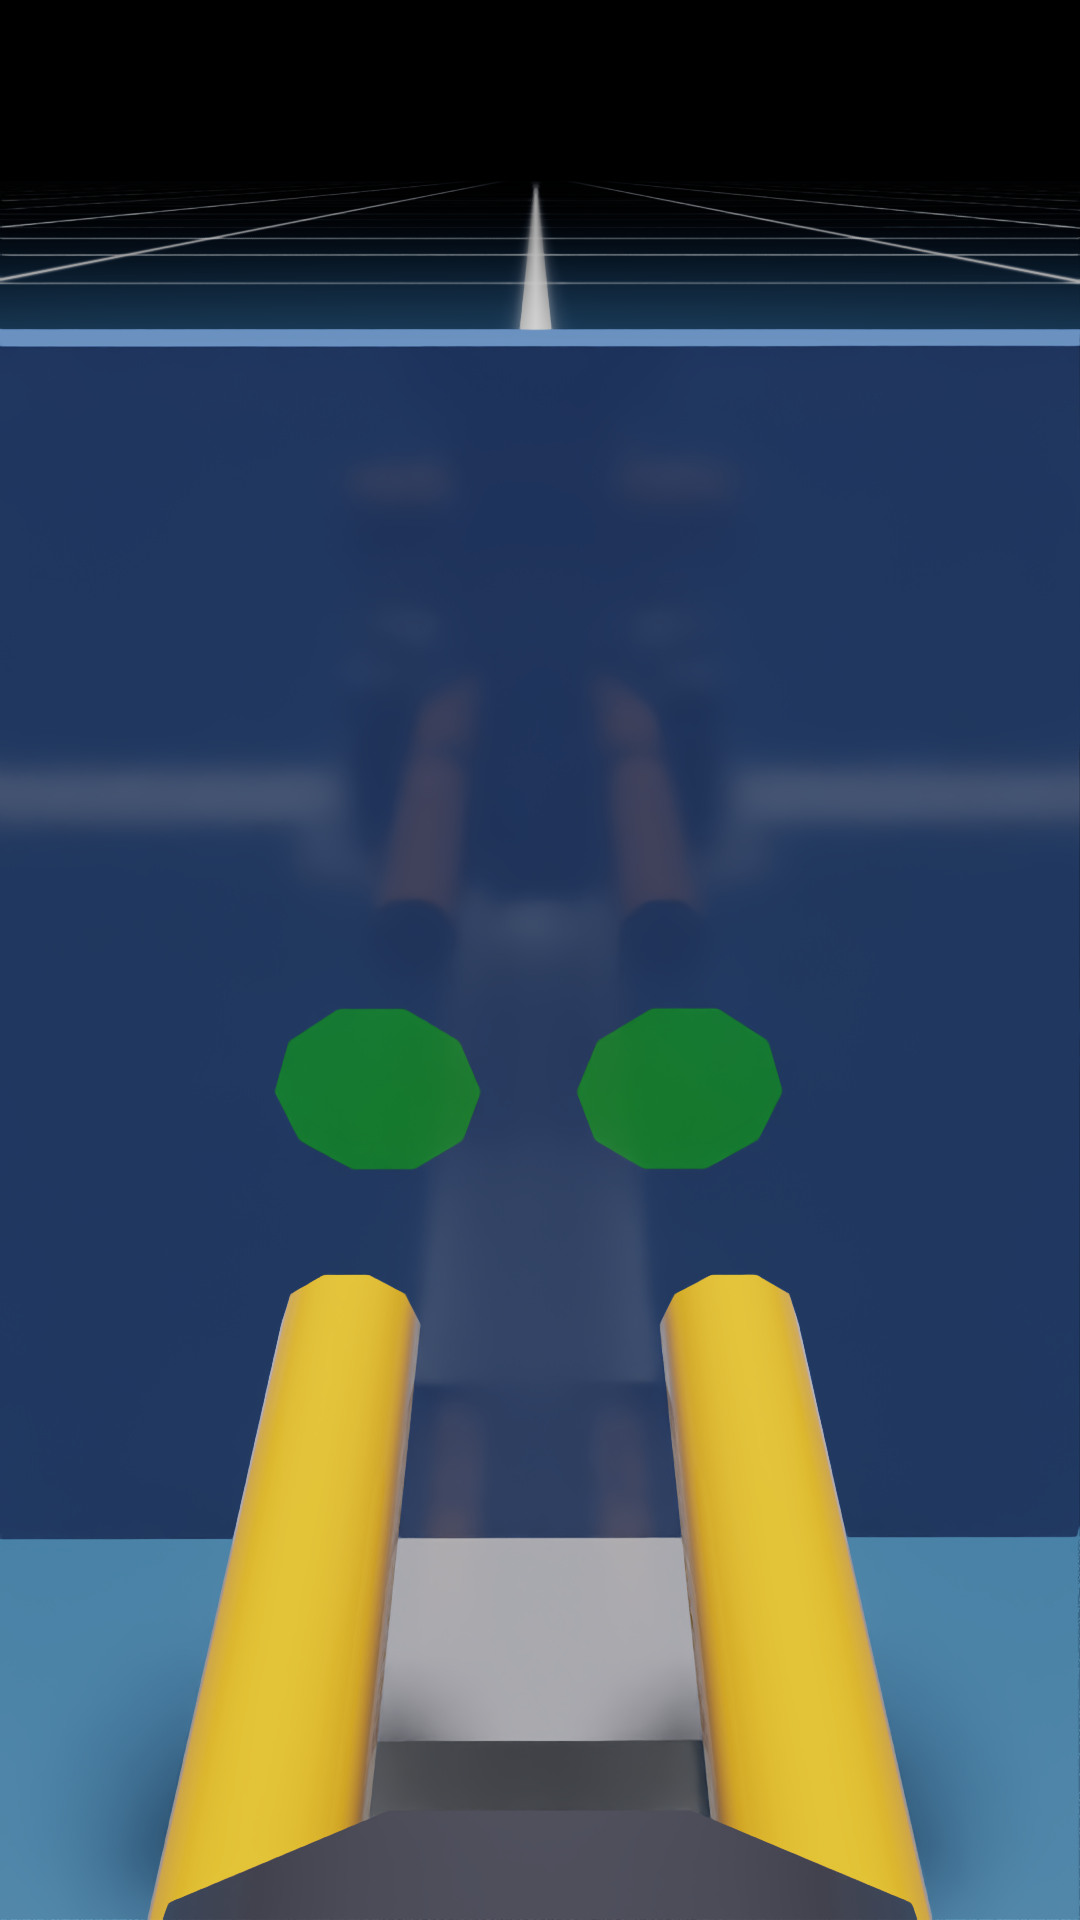
\includegraphics[width=\textwidth]{Figures/report/insertion_step2.png}
  \caption{Visual alignment: plug centred on socket.}
\end{subfigure}
\hfill
\begin{subfigure}[b]{0.23\textwidth}
  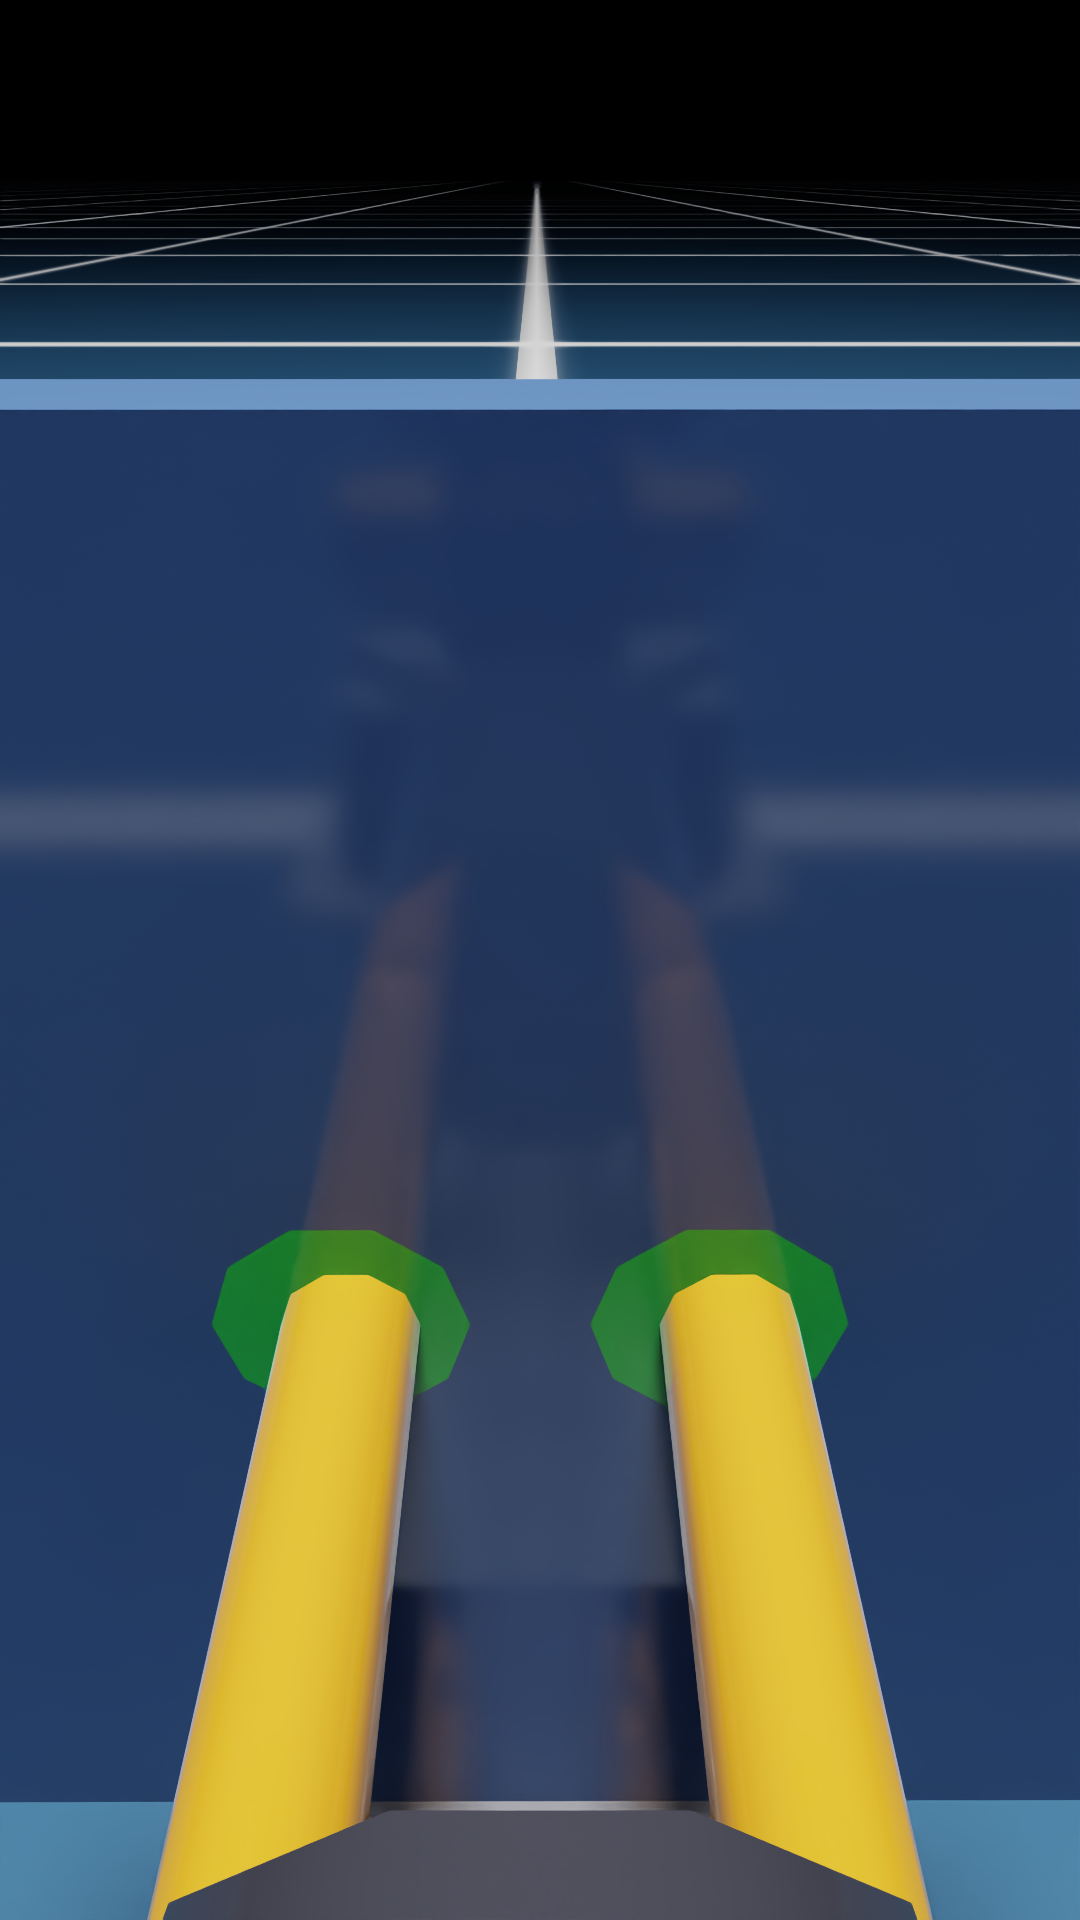
\includegraphics[width=\textwidth]{Figures/report/insertion_step3.png}
  \caption{Initial contact: plug tip at socket face.}
\end{subfigure}
\hfill
\begin{subfigure}[b]{0.23\textwidth}
  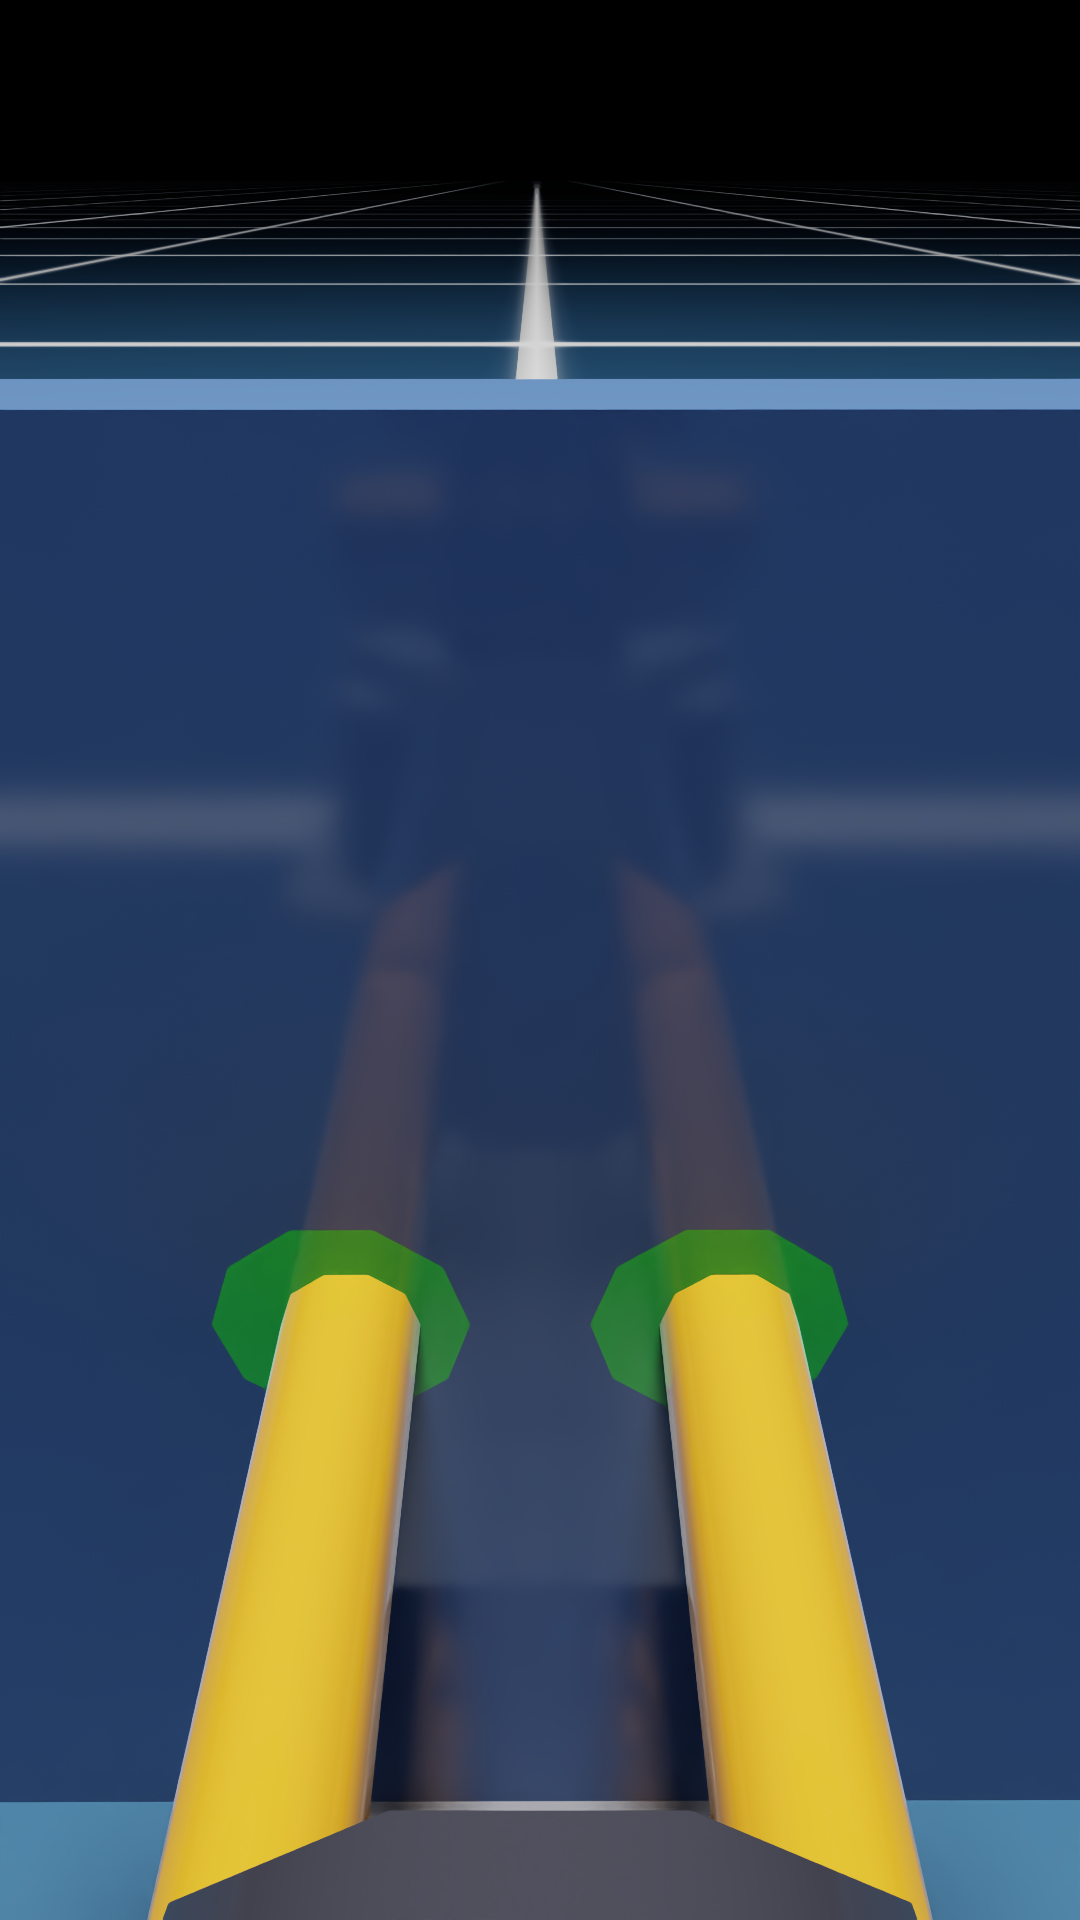
\includegraphics[width=\textwidth]{Figures/report/insertion_step4.png}
  \caption{Fully seated: plug inserted and locked.}
\end{subfigure}
\caption{Required physical evidence for Experiment~7.}
\label{exp:fig:hardware-sequence}
\end{figure}

\textbf{Results to report.} Add a table with the three initial conditions, number of trials, number of successful seating events, success rate, median time to seat, safety-stop count, and observed failure categories. Compare the physical success rate with the matching simulated condition, but do not combine simulator and hardware trials in one success percentage.

\begin{figure}[!htbp]
\centering
\begin{subfigure}[b]{0.48\textwidth}
  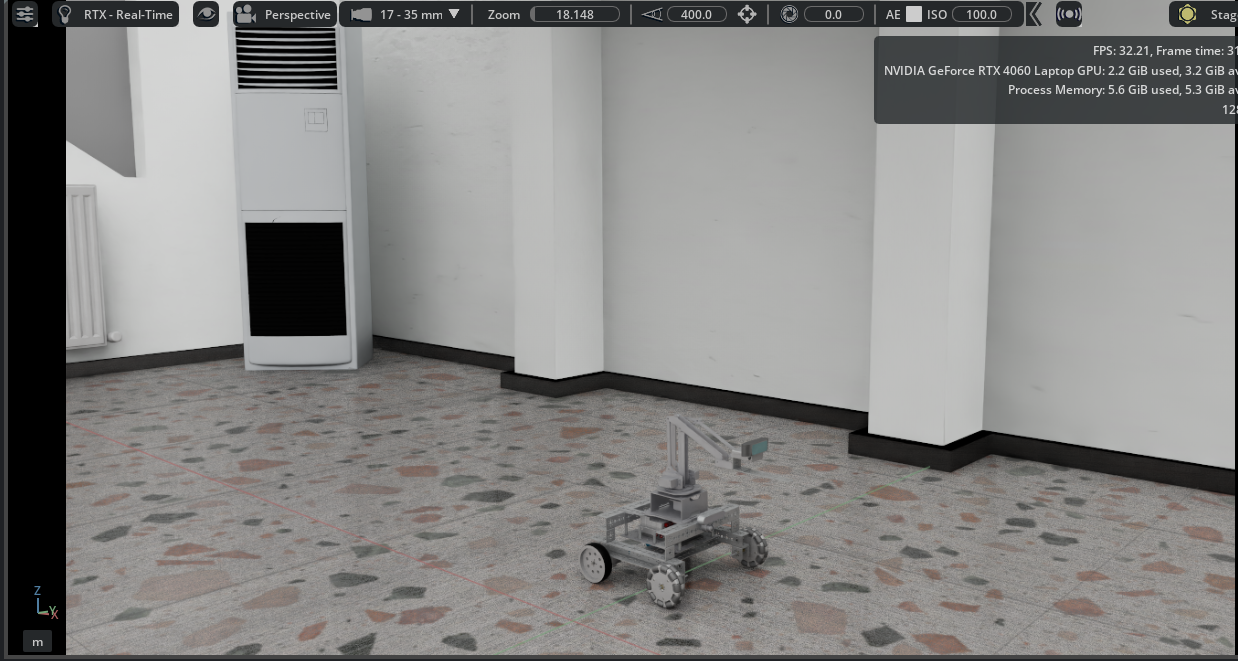
\includegraphics[width=\textwidth]{Figures/report/robot_in_isaac.png}
  \caption{Robot executing insertion in Isaac Sim digital twin.}
\end{subfigure}
\hfill
\begin{subfigure}[b]{0.48\textwidth}
  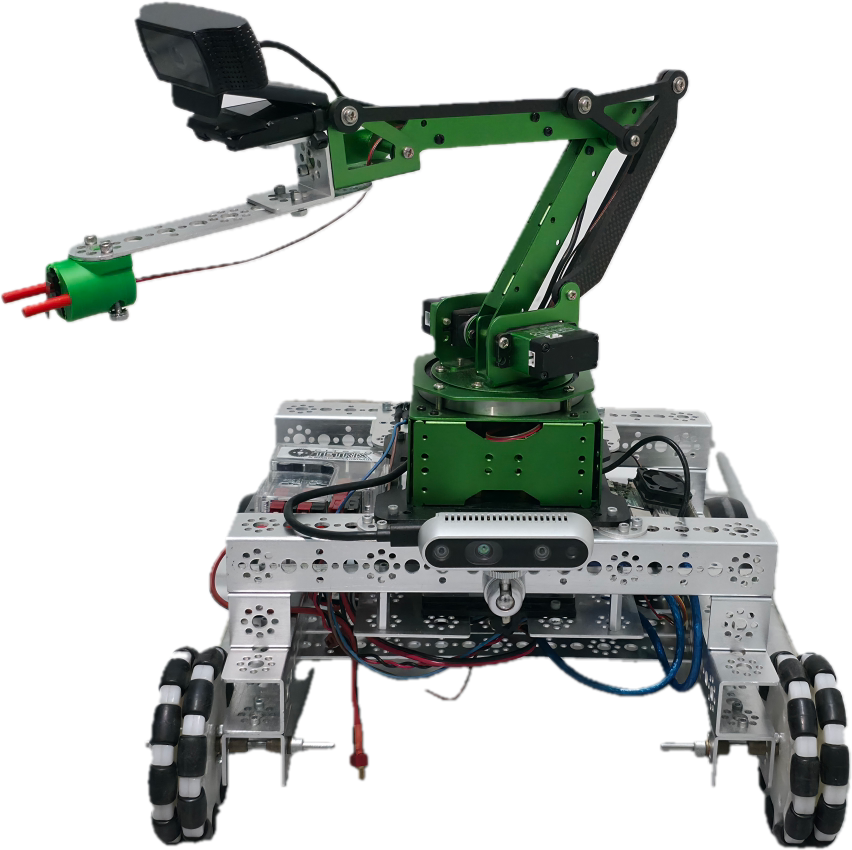
\includegraphics[width=\textwidth]{Figures/report/real_robot1.png}
  \caption{Physical robot performing the same insertion on hardware.}
\end{subfigure}
\caption{Required transfer result for Experiment~7.}
\label{exp:fig:hardware-results}
\end{figure}

\subsection{Experiment 8: End-to-End Autonomous Charging Mission}\label{exp:sec:end-to-end}

\textbf{Purpose.} This experiment demonstrates that the individual modules operate as one system. It tests the complete chain from mobile-base start pose to final plug seating, rather than a manually prepared local insertion scene.

\textbf{Procedure.} Select at least three initial robot locations in the laboratory map and two environmental conditions: clear route and dynamic-object crossing. Run at least five missions per initial location, giving a minimum of \num{15} missions. A mission begins at the documented start pose and ends only when the plug seats or the system enters a safe failure state. Do not manually reposition the base or arm between phases.

For every mission, log the state-machine transitions, SLAM status, navigation result, socket-detection status, final base approach error, arm action trace, seating event, and failure-recovery action. Report phase duration as
\begin{equation}
T_{\mathrm{mission}}=T_{\mathrm{SLAM/nav}}+T_{\mathrm{search}}+T_{\mathrm{align/insert}}.
\label{exp:eq:mission-time}
\end{equation}
This identifies whether any end-to-end failure is caused by navigation, perception, manipulation, or the final insertion policy.


\textbf{Results to report.} Provide a mission table listing success or failure for every phase, total mission success rate, phase durations, number of recovery actions, and failure cause. Discuss the first failed phase, not only the final mission outcome. This preserves the distinction between a navigation failure, a socket-perception failure, and an insertion failure.

\begin{figure}[!htbp]
\centering
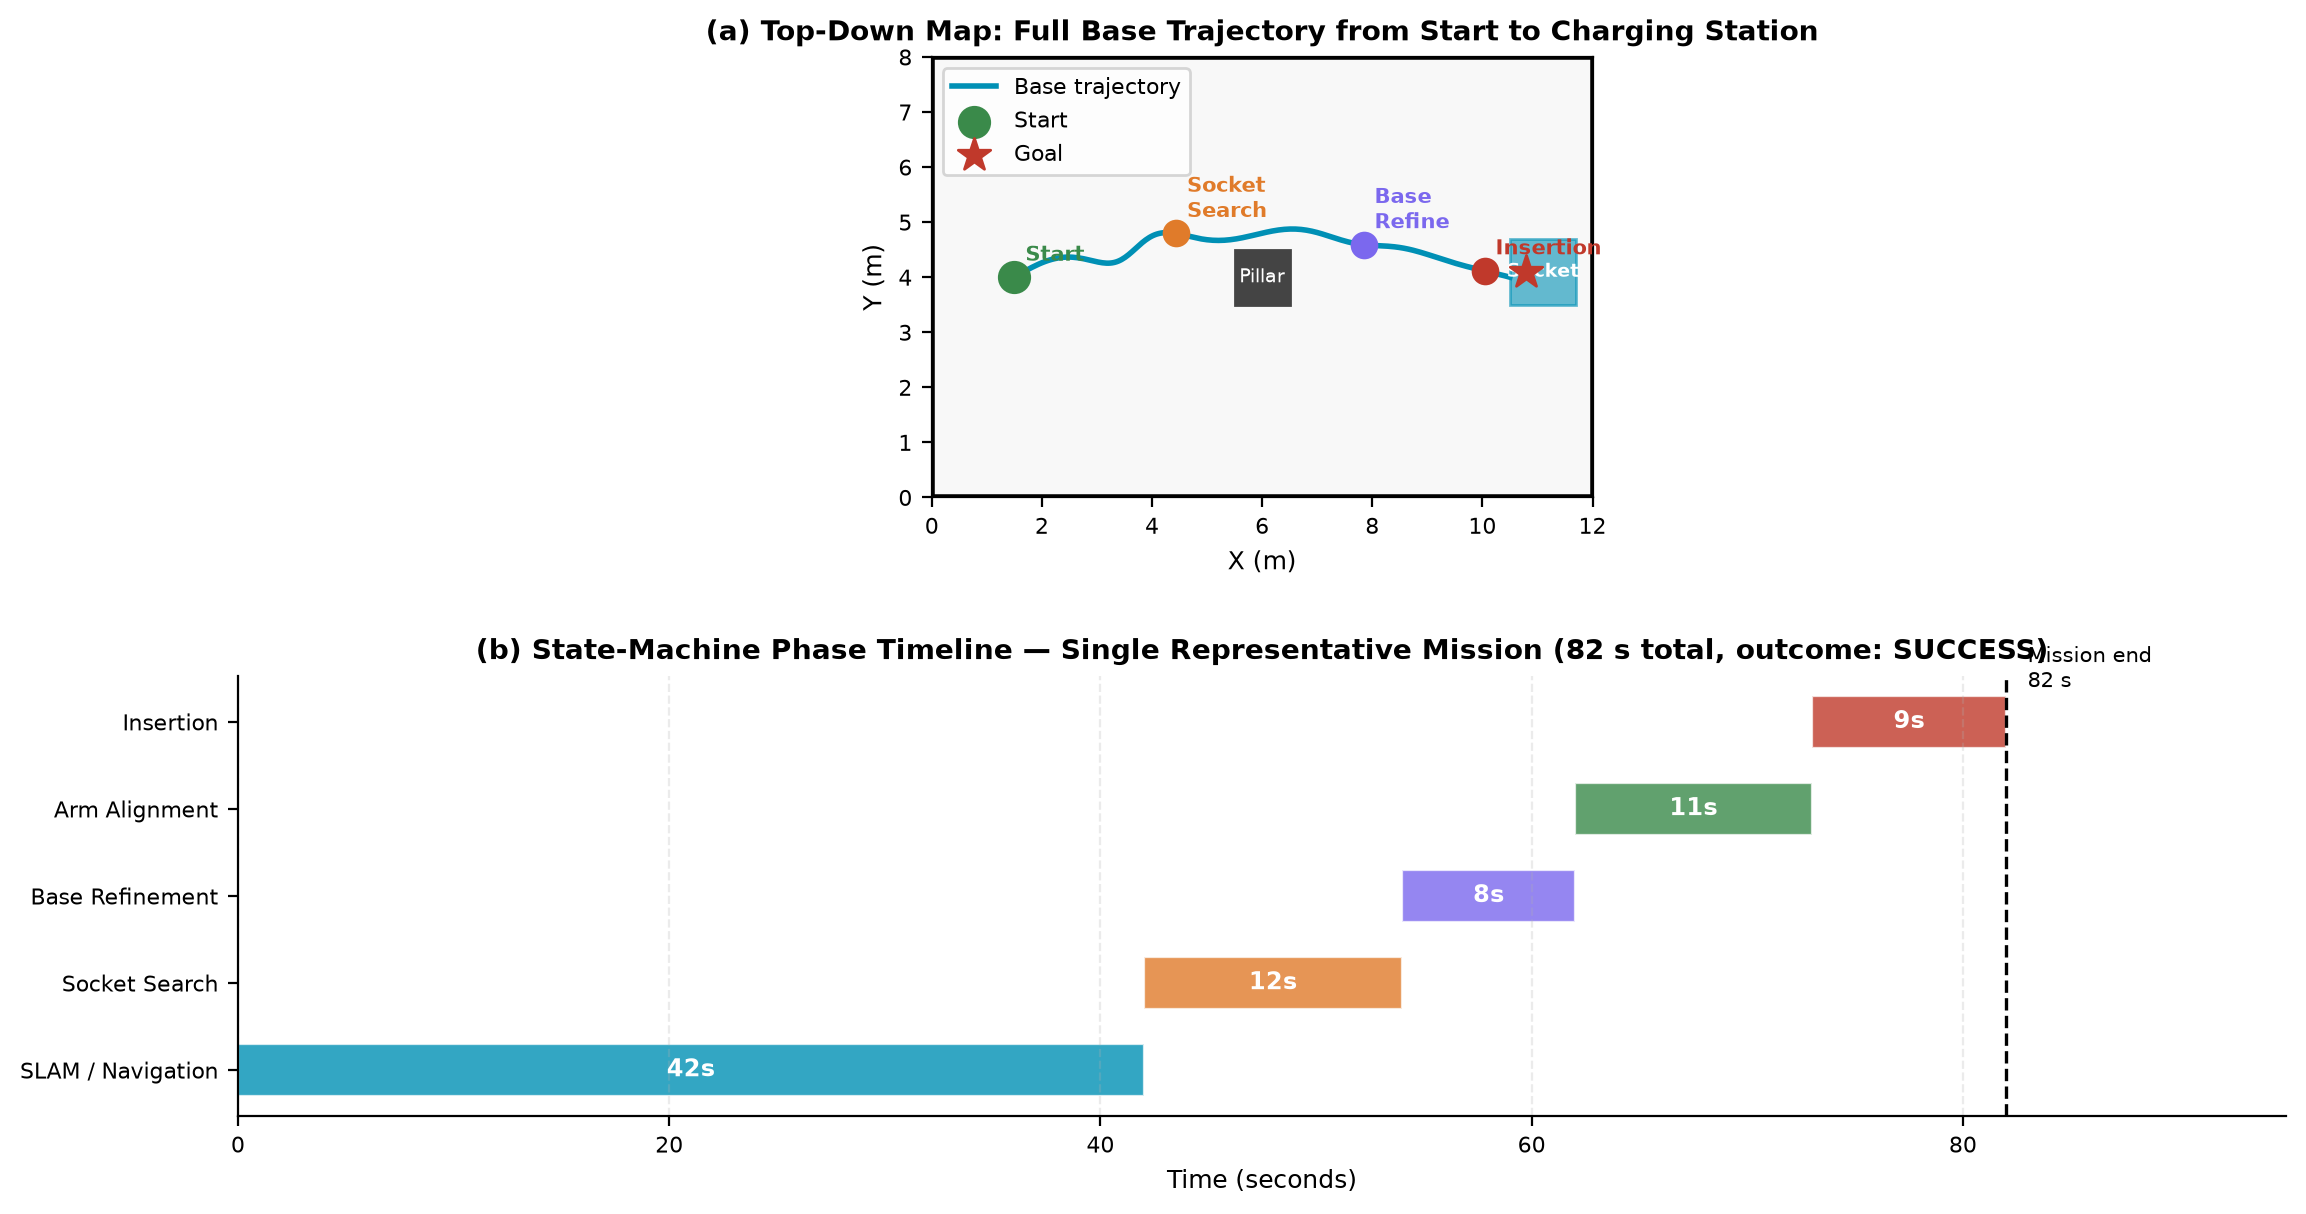
\includegraphics[width=0.96\textwidth]{Figures/report/exp08_timeline.png}
\caption{\textbf{Illustrative figure, not measured data:} generated from assumed values by \texttt{tools/gen\_all\_missing.py} as a stand-in until the experiment is run. End-to-end mission evidence for Experiment~8. (a)~Top-down map showing the base trajectory from the start pose (green circle) to the charging station (red star), with phase change markers overlaid. A pillar obstacle is avoided via the costmap planner. (b)~State-machine phase timeline for a representative successful mission (82\,s total); SLAM and navigation consume the largest share of mission time (42\,s), while base refinement (8\,s) and insertion (9\,s) are comparatively brief.}
\label{exp:fig:end-to-end-trace}
\end{figure}

\subsection{Results Synthesis and Discussion Plan}\label{exp:sec:discussion}

The final discussion should follow the causal order of the system. First, use Experiment~1 to establish whether dynamic visual SLAM provides a stable navigation reference. Next, use Experiments~2--4 to show whether the local perception and motion interfaces provide a repeatable pre-insertion state. Then use Experiments~5--6 to evaluate the contribution and robustness of the learned controller in simulation. Finally, use Experiments~7--8 to state what transfers to hardware and what remains limited by calibration, perception, contact uncertainty, or safety constraints.

Do not use one aggregate success rate to replace this analysis. The report should preserve the per-phase evidence so that a reader can identify where the system succeeds, where it fails, and which design choice is responsible. Table~\ref{exp:tab:summary-results} is the final place to collect the measured values after all experiments are complete.

\begin{table}[!htbp]
\centering
\caption{Final results-summary template. Replace every entry in italics with measured values and retain failed-trial counts.}
\label{exp:tab:summary-results}
\small
\setlength{\tabcolsep}{4pt}
\begin{tabular}{@{}>{\raggedright\arraybackslash}p{0.27\textwidth}>{\raggedright\arraybackslash}p{0.26\textwidth}>{\raggedright\arraybackslash}p{0.37\textwidth}@{}}
\toprule
Experiment & Values to insert & Supported conclusion \\
\midrule
Dynamic visual SLAM & \textit{ATE/RPE, tracking losses, map observation} & \textit{Robustness of localization and mapping} \\
Socket pose estimation & \textit{Detection rate, translation/yaw error} & \textit{Accuracy of the local perception cue} \\
Navigation approach & \textit{Success, approach error, recovery count} & \textit{Reachability of the arm-start pose} \\
Arm positioning & \textit{Position repeatability, orientation error} & \textit{Mechanical/control readiness for insertion} \\
RL simulation & \textit{Accuracy, error distribution, jerk} & \textit{Benefit of PPO over the stated baseline} \\
Robustness ablation & \textit{Performance drop and failure classes} & \textit{Value of domain randomization} \\
Hardware insertion & \textit{Physical success, safety stops, transfer gap} & \textit{Real local-insertion capability} \\
End-to-end mission & \textit{Phase success and mission time} & \textit{Integrated charging-system capability} \\
\bottomrule
\end{tabular}
\end{table}

\endgroup
